\documentclass[a4paper, oneside]{article}

\usepackage{amsmath}
\usepackage{amsthm}
\usepackage{changepage}
\usepackage{amsfonts}
\usepackage{mathpazo}
\usepackage{fancyhdr}
\renewcommand{\footnoterule}{%
  \kern -3pt
  \hrule width \textwidth height 0.4pt
  \kern 2pt
}
\usepackage{color}
\usepackage{perpage} %the perpage package
  \MakePerPage{footnote} %the perpage package command
\usepackage{graphicx}
  \graphicspath{ {./images/} }
\usepackage{float}
\usepackage{hyperref}
\hypersetup{
  colorlinks,
  linkcolor={blue},
  citecolor={blue},
  urlcolor={blue}
}
% \usepackage[margin=1.5in]{geometry}
\usepackage{multicol}
\usepackage{caption}
\usepackage{enumitem}
\usepackage{adjustbox}
\usepackage{array}


%for setting the equation number to sync with the theorem numbers
\numberwithin{equation}{section}
\newcommand{\hint}[1]{\footnote{\raggedleft\rotatebox{180}{Hint: #1\hfill}}}

\rhead{\scshape Apurva Nakade}
\lhead{\scshape Honors Single Variable Calculus 2018}
\renewcommand*{\thepage}{\small\arabic{page}}
\thispagestyle{fancy}

\makeatletter
\def\blfootnote{\xdef\@thefnmark{}\@footnotetext}
\makeatother

\newcommand{\R}{\mathbb{R}}

\theoremstyle{plain}
\newtheorem{theorem}[equation]{Theorem}
\newtheorem{prop}[equation]{Proposition}
\newtheorem{lem}[equation]{Lemma}
\newtheorem{cor}[equation]{Corollary}
\newtheorem{claim}[equation]{Claim}
\newtheorem{axiom}[equation]{Axiom}
\newtheorem{lemma}[equation]{Lemma}

\theoremstyle{definition}
\newtheorem{definition}[equation]{Definition}
\newtheorem{example}[equation]{Example}
\newtheorem{remark}[equation]{Remark}
\newtheorem{note}[equation]{Note}
\newtheorem{exercise}[equation]{Exercise.}
\newtheorem{q}[equation]{Q.}
\newtheorem*{q*}{Q}
\newtheorem*{exercise*}{Exercise}


\newenvironment{indentPara}
    {
    \begin{adjustwidth}{2.5em}{2.5em}
    }
    {
    \end{adjustwidth}
    }

\title{Honors Single Variable Calculus}
\author{Apurva Nakade\\JHU}
\date{}

% \includeonly{08Computations}
\begin{document}
  \cleardoublepage
  \pagenumbering{gobble}
  \maketitle
  \tableofcontents
  \cleardoublepage
  \pagenumbering{arabic}

  %!TEX root=ClassNotes.tex

\section{Proofs}

We'll start by learning about the various kinds of proofs that we'll encounter in this class.\footnote{This section in taken almost verbatim from \url{http://zimmer.csufresno.edu/~larryc/proofs/proofs.html}.}

Proofs are the heart of mathematics. You must come to terms with proofs -- you must be able to read, understand
and write them. What is the secret? What magic do you need to know? The short answer is: there is no secret, no
mystery, no magic. All that is needed is some common sense and a basic understanding of a few trusted and easy
to understand techniques.

\subsection*{The Structure of a Proof}
The basic structure of a proof is easy: it is just a series of statements, each one being either
\begin{itemize}
	\item
	An assumption or
	\item
	A conclusion, clearly following from an assumption or previously proved result
\end{itemize}
And that is all. Occasionally there will be the clarifying remark, but this is just for the reader and has no logical
bearing on the structure of the proof.

A well written proof will flow. That is, the reader should feel as though they are being taken on a ride that takes
them directly and inevitably to the desired conclusion without any distractions about irrelevant details.

Each step
should be clear or at least clearly justified. A good proof is easy to follow.
When you are finished with a proof, apply the above simple test to every sentence: is it clearly
\begin{enumerate}
	\item an assumption
	\item a justified conclusion?
\end{enumerate}
If the sentence fails the test, maybe it doesn't belong in the proof.


\subsection*{Example}
In order to write proofs, you must be able to read proofs. See if you can follow the proof below. Don't worry
about how you would have (or would not have) come up with the idea for the proof. Read the proof with an eye
towards the criteria listed above. Is each sentence clearly an assumption or a conclusion? Does the proof flow?
Was the theorem in fact proved?

\begin{theorem}
	\label{theorem:irrationality_of_sqrt2}
	 The square root of 2 is an irrational number.
\end{theorem}
\begin{proof}
	Let's represent the square root of 2 by $s$. Then, by definition, $s$ satisfies the equation
	\begin{align*}
		s^2 = 2.
	\end{align*}
	If $s$ were a rational number, then we could write $s = p/q$
where $p$ and $q$ are a pair of integers. In fact, by dividing out the common multiple if necessary, we may even assume $p$ and $q$ have no common multiple (other than 1). If we now substitute this into the first equation we obtain, after a little algebra, the equation
\begin{align*}
		p^2 = 2 q^2.
\end{align*}

But now, 2 must appear in the prime factorization of the number $p^2$ (since it appears in the same number $2 q^2$). Since 2 itself is a prime number, 2 must then appear in the prime factorization of the number $p$. But then, $2 \cdot 2$ would appear in the prime factorization of $p^2$, and hence in $2 q^2$. By dividing out a 2, it then appears that 2 is in the prime factorization of $q^2$. Like before (with $p^2$) we can now conclude 2 is a prime factor of $q$. But now we have $p$ and $q$ sharing a prime factor, namely 2. This violates our assumption above (see if you can find it) that $p$ and $q$ have no common multiple other than 1.
\end{proof}

\subsection{Direct Proofs}
Most theorems that you want to prove are either explicitly or implicitly in the form \begin{align*}
	\mbox{ ``If \textit{P}, then \textit{Q}". }
\end{align*} This is the standard form of a
theorem (though it can be disguised). A direct proof should be thought of as a flow of implications beginning
with \textit{P} and ending with \textit{Q}.
	\begin{align*}
		{P} \implies \dots \implies {Q}
	\end{align*}
Most proofs are (and should be) direct proofs. Always try direct proof first, unless you have a good reason not to. If you find a simple proof, and you are convinced of its correctness, then don't be shy about. Many times proofs
are simple and short.

\begin{exercise}
	\label{question:ex1}
	Prove each of the following.
	\begin{enumerate}
		\item If $a$ divides $b$ and $a$ divides $c$ then $a$ divides $b + c$, where $a$, $b$, and $c$ are positive integers.
		\item For all real numbers $a$ and $b$, $a^2 + b^2 \ge 2 a b$.
		\item If $a$ is a rational number and $b$ is a rational number, then $a+b$ is a rational number.
	\end{enumerate}
\end{exercise}



\subsection{Proof by Contradiction}
\label{section:proofByContradiction}
In a proof by contradiction we assume, along with the hypotheses, the logical negation of the result we wish to
prove, and then reach some kind of contradiction. That is, if we want to prove ``If \textit{P}, then \textit{Q}'', we assume \textit{P} and
Not \textit{Q}. The contradiction we arrive at could be some conclusion contradicting one of our assumptions, or
something obviously untrue like 1 = 0. The proof of Theorem \ref{theorem:irrationality_of_sqrt2} is an example of this.

\begin{exercise}
	\label{question:ex2}
	Use the method of Proof by Contradiction to prove each of the following.
	\begin{enumerate}
		\item The cube root of 2 is irrational.
		\item If $a$ is a rational number and $b$ is an irrational number, then $a+b$ is an irrational number.
		\item There are infinitely many prime numbers.\footnote{There are dozens of proofs of this theorem, originally due to Euclid. Feel free to look one up online.}
	\end{enumerate}
\end{exercise}




\subsection{Proof by Contrapositive}
\label{section:proofByContrapositive}
	Proof by contrapositive takes advantage of the logical equivalence between ``\textit{P} implies \textit{Q}'' and ``Not \textit{Q} implies Not \textit{P}''. For example, the assertion ``If it is my car, then it is red'' is equivalent to ``If that car is not red, then it is not mine''. So, to prove ``If \textit{P}, then \textit{Q}'' by the method of contrapositive means to prove
	\begin{align*}
		\mbox{``If Not \textit{Q}, then Not \textit{P}''.}
	\end{align*}

\noindent \textbf{How Is This Different From Proof by Contradiction?}
The difference between the Contrapositive method and the Contradiction method is subtle. Let's examine how the two methods work when trying to prove ``If \textit{P}, then \textit{Q}".
\begin{description}
	\item[Method of Contradiction:] Assume \textit{P} and Not \textit{Q} and prove some sort of contradiction.
	\item[Method of Contrapositive:] Assume Not \textit{Q} and prove Not \textit{P}.
\end{description}
The method of Contrapositive has the advantage that your goal is clear: Prove Not P. In the method of Contradiction, your goal is to prove a contradiction, but it is not always clear what the contradiction is going to be at the start.

\begin{exercise}
	\label{question:ex3}
	Use the method of Proof by Contrapositive to prove each of the following.
	\begin{enumerate}
		\item If the product of two integers is even, then at least one of the two must be even.
		\item If the product of two integers is odd, then both must be odd.
		\item If the product of two real numbers is an irrational number, then at least one of the two must be an irrational number.
	\end{enumerate}
\end{exercise}


\subsection{Converse}
The converse of an assertion in the form ``If \textit{P}, then \textit{Q}" is the assertion
\begin{align*}
	\mbox{``If \textit{Q}, then \textit{P}"}.
\end{align*}
A common logical fallacy is to assume that if an assertion is true then so is its converse.


\subsubsection{If and Only If}
Many theorems are stated in the form ``\textit{P}, if, and only if, \textit{Q}". Another way to say the same thing is: ``\textit{Q} is necessary, and sufficient for \textit{P}". This means two things:
\begin{center}
	``If \textit{P}, Then \textit{Q}" \qquad and \qquad ``If \textit{Q}, Then \textit{P}".
\end{center} So to prove an ``If, and Only If" theorem, you must prove the theorem and also its \textit{converse}.

\begin{exercise}
	Go back to the problems in Exercises \ref{question:ex1}, \ref{question:ex2}, \ref{question:ex3} and find the ones which are of the form ``If \textit{P}, Then \textit{Q}". For each of these:
	\begin{itemize}
		\item State the converse.
		\item Prove or disprove the converse (by providing either a proof or a counterexample).
		\item For the problems where the converse is also true rewrite the assertion as an "If, and Only If" statement.
	\end{itemize}
\end{exercise}








\subsection{Quantifiers}
It is extremely important in mathematics to be able to formulate very precise statements. To prevent ambiguous statements and logical fallacies the vocabulary used is very limited and every term has a well-defined meaning. The two concepts we need to get used to are {\it logical operators} and {\it quantifiers}.\\

{\bf Logical Operators:} Operators allow us to form complex statements by combining simpler ones. The basic logical operators are {\it and}, {\it or}, and {\it not}. Their usage is the same as in everyday language. The more complicated logical operator that we'll be using a lot is {\it If - then -}. We've already encountered several examples of its usage in the previous sections.\\


{\bf Quantifiers:} Quantifiers allow us to make abstract statements which are ``universally true'' without having to specify a concrete element. There are two commonly used	quantifiers:
\begin{align*}
	\mbox{\textbf{For all/every}} && \mbox{\textbf{There exists}}
\end{align*}
Understanding and formulating complex statements using these requires a lot of practice. You'll get used to these as the course progresses. Here are a few examples,
\begin{example}$ $
	\begin{enumerate}
		\item \emph{For every} odd integer $a$, the integer $a+1$ is even.
		\item An integer $a$ is even if and only if \emph{there exists} an integer $b$ such that $a = 2b$.
		\item There \emph{do not exist} integers $p,q$ such that $\frac{p}{q} = \sqrt{2}$.
		\item \emph{For every} non-zero rational number $x$ \emph{there exists} a rational number $y$ such that $x \cdot y = 1$.
	\end{enumerate}
\end{example}

\subsubsection{Nesting Quantifiers}
	When dealing with statements involving multiple quantifiers the order really matters; changing the order changes the meaning of a statement completely. When you're using multiple quantifiers in a single sentence you should always pause and check if you're using the right quantifiers in the right order.

\begin{exercise}
	For each of the following pairs, explain how changing the order of the quantifiers changes the meaning of the statement.\footnote{It's ok to a bit vague in your answers to this question.}
	\begin{enumerate}
		\item \begin{enumerate}
			\item \emph{For every} even integer $a$ \emph{there exists} an integer $b$ such that $a = 2b$.
			\item \emph{There exists} an integer $b$ such that \emph{for every} even integer $a$, $a = 2b$.
		\end{enumerate}
		\item \begin{enumerate}
			\item \emph{For every} positive integer $n$ \emph{there exists} a positive real number $\epsilon$ such that $ \epsilon < 1/n$.
			\item \emph{There exists} a positive real number $\epsilon$ such that \emph{for every} positive integer $n$, $ \epsilon < 1/n$.\footnote{Such an $\epsilon$ is called an {\bf infinitesimal}.	There are number systems, for example the \textbf{hypperreal numbers}, which extend the real numbers by incorporating infinitesimals.}
		\end{enumerate}
		\item \begin{enumerate}
			\item \emph{For every} even integer $a$, \emph{for every} odd integer $b$, $a + b$ is odd.
			\item \emph{For every} odd integer $b$, \emph{for every} even integer $a$, $a + b$ is odd.
			\end{enumerate}
		\item Let $f: \R \rightarrow \R$ be a function and let $\epsilon$ be a positive real number. \begin{enumerate}
			\item {\it For every} $x$, {\it there exists} a $\delta > 0$ such that {\it for every} $y$, if $|x-y| < \delta$ then $|f(x) - f(y)| < \epsilon$.
			\item {\it There exists} a $\delta > 0$ such that {\it for every} $x$, {\it for every} $y$, if $|x-y| < \delta$ then $|f(x) - f(y)| < \epsilon$.
		\end{enumerate}
	\end{enumerate}
\end{exercise}

	\subsubsection{Negating Nested Quantifiers}
	As we saw in Sections \ref{section:proofByContradiction} and \ref{section:proofByContrapositive} we often need to negate mathematical statements.

	In order to systematically negate complicated logical expressions, we observe that we can negate simple statements in the following manner. (These are called {\it De Morgan's laws}.)
	\begin{center}
		\begin{tabular}{|p{0.475\textwidth}|p{0.475\textwidth}|}
			\hline Statement
				&
					Negation \\ \hline & \\
			For every $x$ the statement $P$ is true.
				&
					There exists an $x$ such that the statement $P$ is false.
					\\& \\ \hline &\\
			There exists an $x$ such that the statement $P$ is true.
				&
					For every $x$ the statement $P$ is false.
					\\& \\ \hline &\\
			$P$ is true and $Q$ is true
				&
					$P$ is false or $Q$ is false.
					\\& \\ \hline &\\
			$P$ is true or $Q$ is true
				&
					$P$ is false and $Q$ is false.
					\\& \\ \hline &\\
			If $P$ then $Q$
				&
					$P$ but not $Q$.
					\\& \\ \hline
	\end{tabular}
	\end{center}
	If we have multiple quantifiers in a statement then we start with the outermost quantifier and recursively move inwards.
	\begin{example}
		The negation of {\it ``For every $x$, there exits a $y$ such that, the statement $P$ is true''} equals {\it ``There exists an $x$ such that, for every $y$, the statement $P$ is false.''}
	\end{example}
	\begin{exercise} Negate each of the following.
		\begin{enumerate}
			\item \emph{For every} even integer $a$ \emph{there exists} an integer $b$ such that $a = 2b$.
			\item \emph{There exists} an integer $b$ such that \emph{for every} even integer $a$, $a = 2b$.
			\item \emph{For every} positive integer $n$ \emph{there exists} a positive real number $\epsilon$ such that $ \epsilon < 1/n$.
			\item \emph{There exists} a positive real number $\epsilon$ such that \emph{for every} integer $n$, $ \epsilon < 1/n$.
			\item \emph{For every} even integer $a$, \emph{for every} odd integer $b$, $a + b$ is odd.
			\item {\it For every} $\epsilon > 0$, {\it for every} $x$, {\it there exists} a $\delta > 0$ such that {\it for every} $y$, if $|x-y| < \delta$ then $|f(x) - f(y)| < \epsilon$.
			\item {\it For every} $\epsilon > 0$, {\it there exists} a $\delta > 0$ such that {\it for every} $x$, {\it for every} $y$, if $|x-y| < \delta$ then $|f(x) - f(y)| < \epsilon$.
		\end{enumerate}
	\end{exercise}

	\noindent {\bf Word of caution:} When the word ``and'' is used in a list it is not considered a logical operator (this is a deficiency of the English language). For example, negating the following expression
	\begin{center}
		\emph{For every} even integer $a$ and \emph{for every} odd integer $b$, $a + b$ is odd,
	\end{center}
	does not change the {\it and} to an {\it or} (what happens if you do change the {\it and} to an {\it or}?).

  %!TEX root=ClassNotes.tex

\section{Inequalities}
In this section we'll learn how to solve inequalities and in the process figure out how to write proofs of statements involving inequalities.


The biggest different between equalities and inequalities is that, unlike equalities, there are usually infinitely many (if any) solutions to inequalities. When we we're trying to solve an inequality we're not looking for the best solution, we're not even looking for a good solution, we're simply looking for {\bf one} solution. For example, both $x = 1.001$ and $x = 10^{100}$ are equally valid solutions to the inequality $x > 1$.

\begin{exercise}
	Find a positive real solution to each of the following inequalities.
	\begin{enumerate}
		\item $x ^ 3 + x < 1$
		\item $(1 + x)^2 - 1 < 1$
		\item $1 - (1 - x)^2 < 1$
		\item $x ^ 3 + 2x < 1 + x^2$
		\item $x^{10} + x > 10 $
		\item $x^3 - x > 1$
	\end{enumerate}
\end{exercise}

When we try to solve equalities we try to simply the equation until it becomes easy to solve. The same thing is true for inequalities, however, the ways to simplify an inequality are much more subtle.

\begin{example}
	If we're trying to solve $P(x) > \epsilon$, where $P$ is some complicated expression that cannot be simplified, then we try to find some simpler $Q(x)$, such that $P(x) > Q(x)$ and try to solve for $Q(x) > \epsilon$ instead. Similarly, if we're trying to solve $P(x) < \epsilon$, then we try to find some simpler $Q(x)$, such that $P(x) < Q(x)$ and try to solve for $Q(x) < \epsilon$ instead.

	 There is no {\it canonical way} in which an inequality can be solved. We somehow simplify the inequality and hope that we get a solution.
\end{example}

For solving complicated inequalities, we need a systematic approach towards estimating functions. There are different tricks and identities for estimating different kinds of functions. For now, we'll focus mainly on estimating polynomials.

\begin{exercise}$ $
	\label{q:inequality_1}
	Prove the following extremely useful set of inequalities
	\begin{center}
		\begin{tabular}{ll}
			if $1 \ge x > 0$ &then $ 1 \ge x \ge x^2 \ge x^3 \ge \dots$ \\
			if $1 \le x$ &then $1 \le x \le x^2 \le x^3 \le \dots$.
		\end{tabular}
	\end{center}
\end{exercise}


\noindent {\bf Word of Caution: } You should be very careful when negative numbers are involved. Multiplying an inequality by a negative number changes it's sign, for example, $2 < 3$ but $-2 > -3$. So,
\begin{center}
	\begin{tabular}{ll}
		if $1 \ge x > 0$ &then $ -1 \le -x \le -x^2 \le -x^3 \le \dots$ \\
		if $1 \le x$ &then $-1 \ge -x \ge -x^2 \ge -x^3 \ge \dots$.
	\end{tabular}
\end{center}


\subsection{Proofs involving Inequalities}
We'll encounter several statements in this class like: {\it For every $\epsilon> 0$ there exists a positive real number $x$ such that $x^3 + 3x < \epsilon$.} When we want to prove such a statement, we are essentially trying to solve $x^3 + 3x < \epsilon$. (Why?) For example,\\
\begin{q}
	\label{q:sample_problem_inequality_1}
	Prove that for every $\epsilon > 0$ there exists a positive real number $x$ such that $x^3 + 3x < \epsilon$.
\end{q}
\noindent We're asking for a solution to the equation $x^3 + 3x < \epsilon$ for an arbitrary positive real number $\epsilon$.
\begin{enumerate}
	\item The terms $x^3$ and $x$ have different degrees. We can try to use the inequalities in Exercise \ref{q:inequality_1} to simplify their sum, for this we need to know if $x \ge 1$ or $x \le 1$.
	\item We're probably looking for a small  $x$ so we could assume $x \le 1$. If this does not work we'll come back try something else. (Remember that we're trying to find {\bf one} solution.)
	\item As $x \le 1$, $x^3 \le x$ so that
		$x^3 + 3x \le x + 3x= 4x$.
	\item	As $x^3 + 3x \le 4x$ and we want to find a solution to $x^3 + 3x < \epsilon$, it suffices to solve $4x < \epsilon$. As $\epsilon$ is positive, \textbf{one} solution for this is $x = \epsilon / 5$.
	\item We still need to check if this solution actually works. We can do this by trying to write down a direct proof and making sure that all the implications are logically sound.
	\item We required the condition $x \le 1$ for this solution to work. To ensure this we'll set $x = \min \{ 1, {\epsilon}/{5}\}$.
\end{enumerate}

Now we know what the solution is, but we still need to write down a proof for the original statement. A proof should always start with some assumptions and logically derive the required conclusion. For us the assumption will be $\epsilon > 0$ and $x = \min \{ 1, {\epsilon}/{5}\}$ and the expected conclusion is $x^3 + 3x < \epsilon$.

\begin{proof}[Proof of Q. \ref{q:sample_problem_inequality_1}]
	Let $\epsilon > 0$ and let $x = \min \{ 1, {\epsilon}/{5}\}$. Note that $x \le 1$ and hence $x^3 \le x$. Then,
	\begin{align*}
		x^3 + 3x
		&\le x + 3x \\
		&= 4x \\
		&= 4 \min  \{ 1, {\epsilon}/{5}\} \\
		&\le 4 \epsilon /5 \\
		&< \epsilon & \mbox{ as $\epsilon$ is positive}
	\end{align*}
	Hence, $x= \min \{ 1, {\epsilon}/{5}\}$ is a solution of $x^3 + 3x < \epsilon$, which proves the proposition.
\end{proof}
First we had to solve the inequality then reverse the steps: start with the solution and write a {\it direct proof} for the proposition. This is how proofs are usually discovered. You make an ``educated guess'' and hope that it works. Sometimes it doesn't, so you go back to finding another ``educated guess''.


\begin{remark}[A note on quantifiers]
	 For proving the statement {\it``prove that for every $\epsilon > 0$ there exists a positive real number $x$ such that $x^3 + 3x < \epsilon$''} we had to start with the statement {\it ``let $\epsilon > 0$ and $x = \min \{ 1, {\epsilon}/{5}\}$''}.
	 The variable $x$ depends on the variable $\epsilon$.
	 This is fine because of the order of quantifiers: {\it``\dots for every $\epsilon > 0$ there exists a positive real number $x$ \dots''}; the quantifier for $\epsilon$ comes before the quantifier for $x$ and hence the variable $x$ can depend on the variable $\epsilon$.

	If instead, suppose we were trying to prove {\it ``there exists a positive real number $x$ such that for every $\epsilon > 0$, $x^3 + 3x < \epsilon$''}.
	We're still trying to solve the equation $x^3 + 3x < \epsilon$ but now the quantifier for $x$ comes before the quantifier for $\epsilon$ and hence $x$ cannot depend on the variable $\epsilon$ but instead should be a constant that universally solves the equation $x^3 + 3x < \epsilon$ for every $\epsilon > 0$.
	No such $x$ exists (why?) and hence the statement {\it ``there exists a positive real number $x$ such that for every $\epsilon > 0$, $x^3 + 3x < \epsilon$''} is false.
\end{remark}

\begin{exercise}
	Prove that for every $\epsilon > 0$ there exists a positive real number $x$ such that \dots
		\begin{enumerate}
			\item  $x ^ 3 + x < \epsilon$.
			\item  $(1 + x)^2 - 1 < \epsilon$.
			\item $1 - (1 - x)^2 < \epsilon$.
			\item  $x ^ 3 + 2x < \epsilon + x^2$.
			\item  $x^{10} + x > \epsilon $.
			\item  $x^3 - x > \epsilon $.
						\hint{Break $x^3$ as $\frac{x^3}{2} + \frac{x^3}{2}$ and find the conditions on $x$ for which $\left(\frac{x^3}{2} - x\right) > 0$.}\\
		\end{enumerate}
\end{exercise}

Finally, we are sometimes required to find not one solution but a range of solutions. We try to come up an ``educated guess'' by the same method, and many a times this gives us the required range for free with a few changes in the final proof.

\begin{q}
	\label{q:sample_problem_inequality_2}
	Prove that for every $\epsilon > 0$, there exists a positive real number $\delta$ such that, for all $x$, if $0 < x < \delta$ then $x^3 + 3x < \epsilon$.
\end{q}
\begin{proof}
	Let $\epsilon > 0$, let $\delta = \min \{ 1, \epsilon/5\}$ and let $ 0 < x < \delta$. Because $\delta \le 1$, we have $x < 1$ and hence $x^3 < x$. As before,
	\begin{align*}
		x^3 + 3x
		&\le x + 3x \\
		&= 4x \\
		&< 4 \delta \\
		&= 4 \min  \{ 1, {\epsilon}/{5}\} \\
		&\le 4 \epsilon /5 \\
		&< \epsilon& \mbox{ as $\epsilon$ is positive}
	\end{align*}
	Hence, every $0 < x <  \min \{ 1, \epsilon/5\}$ is a solution of $x^3 + 3x < \epsilon$, which proves the proposition.
\end{proof}


\begin{exercise}
	Prove that for every $\epsilon > 0$, there exists a positive real number $\delta$ such that, for all $x$, if $ 0 < x < \delta$ then \dots
		\begin{enumerate}
			\item  $x ^ 3 + x < \epsilon$.
			\item  $(1 + x)^2 - 1 < \epsilon$.
			\item $1 - (1 - x)^2 < \epsilon$.
			\item  $x ^ 3 + 2x < \epsilon + x^2$.
		\end{enumerate}
		\noindent Prove that for every $\epsilon > 0$, there exists a positive real number $\delta$ such that, for all $x$, if $ x > \delta$ then
		\begin{enumerate}
			\item $x^{10} + x > \epsilon $.
			\item $x^3 - x > \epsilon$.
		\end{enumerate}
\end{exercise}

\subsubsection*{Optional Problems}
\begin{exercise}
	\begin{enumerate}
		\item Prove that for every $\epsilon > 0$, for every real number $x > 0$, there exists a $\delta > 0$ such that, for all real numbers $y > 0$, if $ 0 < y - x < \delta$ then $y^2 - x^2 < \epsilon$.
		\item Prove that the following statement is false: For every $\epsilon > 0$, there exists a $\delta > 0$ such that, for every real number $x > 0$, for all real numbers $y > 0$, if $ 0 < y - x < \delta$ then $y^2 - x^2 < \epsilon$.
	\end{enumerate}
\end{exercise}

  %!TEX root=ClassNotes.tex
\section{Limits \& Continuity}

We'll now use the proof techniques we've learned so far to study functions.

We'll start with rigorously defining limits. At first this might seem unnecessarily complicated, but having precise definitions will allow us to make more and more sophisticated constructions and later on in the course enable us to prove statements about derivatives and integrals.

Time permitting, towards the end of the semester, we'll construct the Weierstrass function, a function defined on real numbers which is continuous everywhere but differentiable nowhere! But it all starts with the definition of a limit.

\begin{figure}[H]
	\centering
	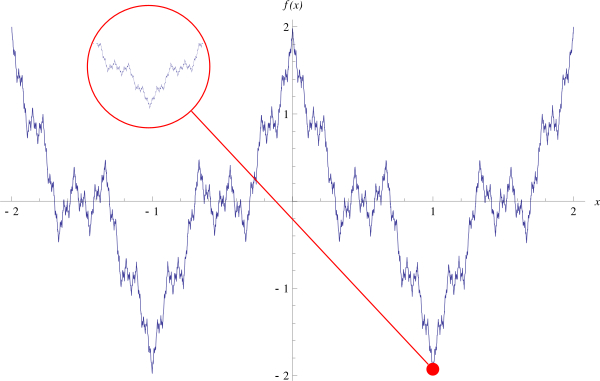
\includegraphics[width=0.6\textwidth]{WeierstrassFunction.jpg}
	% \captionsetup{labelformat=empty}
	\caption*{Weierstrass function (Image from Wikipedia)}
\end{figure}

\subsection{Limits}
At the heart of all analysis (and hence calculus) lies the notion of a limit. Almost every single concept that we'll define will be a limit of some kind.

\begin{definition}[Provisional definition of limit]
	\label{def:provisional_definition_limit}
	For a function $f$ and a real number $a$, we say that the function $f$ \textbf{approaches a limit $L$ at $a$}, for some real number $L$, if we can make $f(x)$ as close to $L$ as we like by requiring that $x$ be sufficiently close to, but unequal to, $a$. This is denoted
	\begin{align*}
		\lim \limits _ {x \rightarrow a} f(x) = L
	\end{align*}
\end{definition}
\noindent There are 3 problems with this definition:
\begin{enumerate}
	\item The terms {\it ``as close to $L$ as we like''} and {\it``sufficiently close''} are not precise. (How close is sufficiently close?)
	\item The order of implication is unclear.
	\item The definition does not give us a way to come up with the limit $L$.
\end{enumerate}

First, we'll make the terms precise.  We can measure the distance between two real numbers $x$, $y$ by taking their difference $x - y$, however, the difference can be negative so we use the absolute value $|x - y|$ instead.  So that
\begin{center}
	\begin{tabular}{l l l}
		{\it $x$ sufficiently close to, but unequal to, $a$} & translates to & {\it $0 < |x - a| < \delta$}                            \\
		{\it $f(x)$ as close to $L$ as we like}              & translates to & {\it for every $\epsilon > 0$, $|f(x) - L| < \epsilon$}\end{tabular}
\end{center}
and the definition of limit becomes\\
\begin{indentPara}
	\dots $f$ \textbf{approaches a limit $L$ at $a$}, for some real number $L$, if we can make $|f(x) - L| < \epsilon$ for every $\epsilon > 0$ by requiring that $0 < |x - a | < \delta$ for some $\delta > 0$.\\
\end{indentPara}

Next, to clarify the order of implication we rephrase the statement in the more standard {\it ``If ... then''} form and put all the quantifiers in the front,\\
\begin{indentPara}
	\dots $f$ \textbf{approaches a limit $L$ at $a$}, for some real number $L$, if for every $\epsilon > 0$, there exists a $\delta > 0$ such that, for all $x$, if $0 < |x - a | < \delta$ then $|f(x) - L| < \epsilon$.\\
\end{indentPara}


The third problem cannot be fixed! There is no systematic way of finding the limit of a general function, the only thing we can do is {\it guess} the limit and then use the definition to {\it prove} that it is indeed the limit. For special functions like polynomials, trig functions, exponential, and logarithms, we can find limits explicitly, which is what makes these functions useful for approximating and estimating more complicated functions.

\begin{definition}[Formal definition of limit]
	\label{def:formal_definition_limit}
	We say that the function $f$ \textbf{approaches a limit $L$ at $a$}, for some real number $L$, if for every $\epsilon > 0$, there exists a $\delta > 0$ such that, for all $x$, if $0 < |x - a | < \delta$ then $|f(x) - L| < \epsilon$.
\end{definition}

\begin{exercise}
	Come up with formal definitions for the following:
	\begin{enumerate}
		\item The function $f$ approaches a limit $L$ at $a$ {\bf from the right}, for some real number $L$, if we can make $f(x)$ as close to $L$ as we like by requiring that $x$ be sufficiently close to, but strictly greater than $a$. This is denoted
		      \begin{align*}
			      \lim \limits _ {x \rightarrow a^+} f(x) = L.
		      \end{align*}
		\item The function $f$ approaches a limit $L$ at $a$ {\bf from the left}, for some real number $L$, if we can make $f(x)$ as close to $L$ as we like by requiring that $x$ be sufficiently close to, but strictly smaller than $a$. This is denoted
		      \begin{align*}
			      \lim \limits _ {x \rightarrow a^-} f(x) = L.
		      \end{align*}
		\item The function $f$ \textbf{approaches the limit $\infty$ at $a$}, if $f(x)$ can be made as large as we like by requiring that $x$ be sufficiently close to, but unequal to, $a$. This is denoted \footnote{
		In mathematics $\infty$ means several things, in fact, there are infinitely many infinities. For us, $\infty$ is a {\it placeholder} for a limit of a function that grows very large. $\infty$ is not a real number and hence cannot be used in equations.}
		      \begin{align*}
			      \lim \limits _ {x \rightarrow a} f(x) = \infty.
		      \end{align*}

		\item The function $f$ \textbf{approaches a limit $L$ at $\infty$}, for some real number $L$ if we can make $f(x)$ as close to $L$ as we like by requiring that $x$ be sufficiently large. This is denoted
		      \begin{align*}
			      \lim \limits _ {x \rightarrow \infty} f(x) = L.
		      \end{align*}
		% \item The function $f$ \textbf{does not approaches a limit $L$ at $a$}. Further generalize this to: the function $f$ does not approaches a limit $L$ at $a$, {\it for any $L$}. In this case, we say that the {\bf limit of $f$ at $a$ does not exist}.
	\end{enumerate}
\end{exercise}

\begin{exercise}
	For each of the following, first guess the limit, then use the formal definition of limit to prove that it is indeed the limit.
	\begin{enumerate}
		\item $\lim \limits_{x \rightarrow 1^+} 2x + 1$
		\item $\lim \limits_{x \rightarrow 1^+} x^2$
		\item $\lim \limits_{x \rightarrow \infty} x^{10} + x$
		\item $\lim \limits_{x \rightarrow 0^+} 1/x$
		% \item $\lim \limits_{x \rightarrow 0^+} \dfrac{\sin x}{x}\qquad$  (You can assume that $\sin x < x - \dfrac{x^3}{6}$ for all $0 < x < 1$.)
		\item $\lim \limits_{x \rightarrow 0} f(x)$ where $f(x) = \begin{cases}
				      x & \mbox{ if $x$ is rational}   \\
				      0 & \mbox{ if $x$ is irrational}
			      \end{cases}$
	\end{enumerate}
\end{exercise}

\subsubsection*{Optional Problems}

\begin{exercise} Give examples to show that the following definitions of $\lim \limits _ {x \rightarrow a} f(x) = L$ are not correct.
	\begin{enumerate}
		\item For every $ \delta > 0$, there exists an $ \epsilon > 0$ such that, for all $x$, if $ 0<|x-a|< \delta$ then $ |f(x) - L|< \epsilon$.
		\item For every $\epsilon > 0$, there exists a $\delta > 0$ such that, for all $x$, if $|f(x) - L| < \epsilon$ then $0 < |x - a| < \delta$.
	\end{enumerate}
\end{exercise}

\begin{exercise}
	Prove that if $\lim \limits _ {x \rightarrow a} f(x) = L$ and $ L \neq 0$ then $\lim \limits _ {x \rightarrow a} 1/f(x) = 1/L$ .
\end{exercise}



\subsubsection{Triangle Inequality}

To prove abstract theorems involving absolute values we will need the following very important inequality called the {\bf triangle inequality}.
\begin{align*}
	|x - y| \le |x| + |y|
\end{align*}
If you think of the points $0$, $x$, $y$ (on the real axis) as being the three vertices of a (degenerate) triangle, then $|x|$, $|y|$, and $|x - y|$ are the lengths of the three sides and the triangle inequality is saying that: {\it the sum of the lengths of two sides of a triangle is greater than or equal to the length of the third side.}\\\\
There are other forms in which the triangle inequality is commonly used, e.g.
\begin{align*}
	|x + y|       & \le |x| + |y|   \\
	|x + y| - |y| & \le |x|         \\
	|x|           & \le |x-y| + |y|
\end{align*}
These inequalities are central to a lot of analysis proofs.

\begin{exercise}$ $
	\begin{enumerate}
		\item Prove that $|x| + |x - 1| \ge 1$ for any real number $x$.
		\item Prove that for any real number $x$, at least one of $|x|$ and $|x-1|$ is $\ge 1/2$.\hint{Proof by Contradiction.}
	\end{enumerate}
\end{exercise}

We'll use these to prove inequalities about the non-existence of limits.

\begin{definition}
	If $f$ does not approach the limit $L$, for any real number or $\infty$ or $-\infty$, then we say that the limit of $f$ at $a$ {\bf does not exist}.
\end{definition}

\begin{exercise}
	\label{q:formal_definition_non_existence_limit}
	Negate the formal definitions of limits and come up with an $\epsilon, \delta$ definition for the following.
	\begin{enumerate}
		\item $f$ {\bf does not} approach the limit $L$, where $L$ is a real number, at $a$.
		\item $f$ {\bf does not} approach the limit $\infty$ at $a$. (Similarly for $-\infty$.)
	\end{enumerate}
\end{exercise}

\begin{exercise}
	\label{q:rational_irrational_discontinuity}
	Let $
		f(x) = \begin{cases}
			1 & \mbox{if $x$ is rational,}   \\
			0 & \mbox{if $x$ is irrational.}
		\end{cases}
	$
	\begin{enumerate}
		\item Prove that for every real number $L$, $\lim \limits_{x \rightarrow 0} f(x) \neq L$.
		\item Prove that $\lim \limits_{x \rightarrow 0} f(x) \neq \infty$. (Similarly for $-\infty$.)
	\end{enumerate}
	Hence the limit of $f$ at $0$ does not exist.
\end{exercise}

\begin{exercise}$ $
	\begin{enumerate}
		\item Prove that $\lim \limits_{x \rightarrow a} f(x) = L$ if and only if $\lim \limits_{x \rightarrow a^+} f(x) = L$ and $\lim \limits_{x \rightarrow a^-} f(x) = L$.\hint{This is very easy, don't overthink! Simply write down the formal definitions.}
		      (Similarly for $\infty$, $-\infty$.)

		\item Prove that $\lim \limits_{x \rightarrow 0} \dfrac{1}{x}$ does not exist.
	\end{enumerate}
\end{exercise}


\subsection{Non-existence of limits}

Let's move backwards and try and understand what it means {\it intuitively} for a function to not approach a limit $L$ near $a$. The solution to Exercise \ref{q:formal_definition_non_existence_limit} is the following:\\

\begin{indentPara}
	{\it (Formal definition)} The function $f$ \textbf{does not approach thelimit $L$ at $a$} if there exists an $\epsilon > 0$, such that for all $\delta > 0$, there exists an $x$ such that, $0 < |x - a | < \delta$ and $|f(x) - L| \ge \epsilon$.\\
\end{indentPara}

Going back to how to we came up with the Formal Definition of Limit 	\ref{def:formal_definition_limit}
from the Provisional Definition of Limit \ref{def:provisional_definition_limit} and replacing the absolute values by the distance between points, we can work backwards and get the following provisional definition:\\

\begin{indentPara}
	{\it (Provisional definition)}
	The function $f$ \textbf{does not approach the limit $L$ at $a$} if no matter how close we are to $a$, there is some $x$ for which $f(x)$ is not close to $L$.
\end{indentPara}


% \subsubsection*{Optional Problems}
% \begin{exercise} $ $
% 	\begin{enumerate}
% 		\item Explain how the provisional definition captures the notion of the failure of the function to approach a limit $L$ at $a$.
% 		\item Starting from the provisional definition try to systematically come up with the formal definition using arguments similar to the ones we made to go from Definition  \ref{def:provisional_definition_limit} to Definition \ref{def:formal_definition_limit}.
% 	\end{enumerate}
% \end{exercise}
%
% \begin{exercise}
% 	It is easy to show that for the function
% 	\begin{align*}
% 		f(x) = \begin{cases}
% 			0 & \mbox{if } x \le 0 \\
% 			1 & \mbox{if } x > 0
% 		\end{cases}
% 	\end{align*}
% 	the limit $\lim \limits_{x \rightarrow 0} f(x)$ does not exist by computing the limits from the left and the right.
%
% 	Try to prove that, $\lim \limits_{x \rightarrow 0} f(x) \neq L$ for some real numbers, say $L = 0$, 1, 1/2, and more generally for any real number, using the formal definition and try to explain what the variables $\epsilon$, $\delta$, $x$ in your proof mean {\it geometrically}.
% \end{exercise}

\subsection{Continuity}

\begin{definition}
  We say that a function $f$ is {\bf continuous} at $a$ if
  \begin{align*}
    \lim \limits_{x \rightarrow a} f(x) = f(a)
  \end{align*}
  We say that a function $f$ is {\bf continuous on an interval} $(a,b)$ it $f$ is continuous at every $x$ in $(a,b)$. \footnote{If we use closed intervals $[a,b]$ instead, then we have to use $\lim \limits_{x \rightarrow a^+}$ and $\lim \limits_{x \rightarrow b^-}$ in the definition of continuity.}
\end{definition}

Thus continuous functions have {nice} limits. Further, we have the following theorem which makes continuous functions easy to manipulate.

\begin{theorem}
  \label{theorem:continuous_functions}
  If the functions $f$, $g$ are continuous at $x=a$ then so are the functions
  \begin{enumerate}
    \item $ f + g$
    \item $f \cdot g$
    \item $f / g$, if $g(a) \neq 0$
  \end{enumerate}
\end{theorem}

\noindent The full proof of this theorem is just a tricky application of the triangle inequalities. We'll only prove the first part which is relatively manageable.


\begin{exercise}
  \label{q:for_later_1}
  Using the formal definition of limits and the triangle inequality $|x+y| \le |x| + |y|$, prove that
  \begin{indentPara}
    {\it if the functions $f$, $g$ are continuous at $x=a$ then so is the function $f + g$.}
  \end{indentPara}
  Is the converse true?
\end{exercise}

\begin{exercise}$ $
  \label{q:for_later_2}
  \begin{enumerate}
    \item Prove that the constant function $f(x) = c$ is continuous everywhere, where $c$ is some real number.
    \item  Prove that the function $f(x) = x$ is continuous everywhere.
    \item Argue that these two facts along with Theorem \ref{theorem:continuous_functions} imply that polynomials are continuous everywhere.
  \end{enumerate}
\end{exercise}

\begin{exercise}
  \label{q:for_later_3}
  Let $f$ be a continuous function on $[a,b]$, and let $g$ be a continuous function on $[b,c]$, such that \begin{align*}
    f(b) = g(b).
  \end{align*}
  Show that the function $h$ defined as
  \begin{align*}
    h(x) :=
    \begin{cases}
      f(x) & \mbox{if } x \le b \\
      g(x) & \mbox{if } x > b
    \end{cases}
  \end{align*}
  is continuous at $b$ (i.e. we can {\it glue} continuous functions).
\end{exercise}

  %!TEX root=ClassNotes.tex

\section{Completeness of the Real Numbers}
Our next goal is to prove the IVT for continuous functions.

\begin{theorem}[Intermediate Value Theorem]
	If $f$ is a continuous function on $[a,b]$ and $k$ is a real number lying between $f(a)$ and $f(b)$ then there exists a real number $ c $ lying between $a$ and $b$ such that $f(c) = k$.
\end{theorem}

The proof of this trivial looking theorem relies on a defining axiom of the system of real numbers called {\it completeness} which we'll now try to understand. For this we'll need to rigorously define the simple notions of {\it min} and {\it max}.\\


For a non-empty set $S$ of real numbers, it's maximum element can be defined as follows.
\begin{definition}
	\label{def:maximum}
	$\max S$ is the element $a \in S$ such that $a \ge x$ for all elements $x \in S$.
\end{definition}
This definition exposes a subtle shortcoming of $\max S$. It doesn't exist even for {\it nice} sets.
\begin{exercise}
	What is $\max \: (0,1)$? Make sure that your answer agrees with Definition \ref{def:maximum}.
\end{exercise}

There is a more intricately defined number, called the {\bf supremum}, that we can associate to a set of real numbers which also captures the {\it largest-element} property. For sets containing infinitely many elements, the supremum, rather than the maximum gives us the correct {\it largest-element}.

\begin{definition}
	An {\bf upper bound} of a set $S$ is any real number $a$ satisfying $a \ge x$ for all elements $x \in S$. (Note that $a$ does not have to be in $S$.)
\end{definition}

\begin{exercise}
	\label{q:upper_bounds}
	Upper bounds are not unique. Find all the possible upper bounds on the following sets. (No proofs needed. Make sure you've found {\it all} the upper bounds.)
	\begin{enumerate}
		\item $[0,1]$
		\item $(0,1)$
		\item $\R$
		\item $\{ 1/n :$ where $n$ is a positive integer$\}$
		\item The set of rational numbers $x$ satisfying $x^2 < 2$
		\item The set of irrational numbers in interval $[0,1]$.
	\end{enumerate}
\end{exercise}

\begin{definition}
	The {\bf supremum} or the {\bf least upper bound} of a set $S$ of real numbers, denoted $\sup S$, is the smallest real number $a$ such that $a$ is an upper bound of $S$.
\end{definition}

\begin{exercise}
	Find the supremum of the sets in Exercise \ref{q:upper_bounds}.
\end{exercise}


\begin{definition}
	We say that a set $S$ is {\bf bounded from above} if it has at least one upper bound i.e. there exists a real number $a$ such that $a \ge x$ for all elements $x \in S$.
\end{definition}

\begin{exercise}
	Which of the sets in Exercise \ref{q:upper_bounds} are bounded from above?\\
\end{exercise}

We can now state the {\bf Completeness of the Real Numbers}:
\begin{theorem}
	If a non-empty set $S$ is bounded from above then $S$ has a supremum.
\end{theorem}

Depending on exactly how the real numbers are constructed, this is either a theorem or an axiom. This theorem/axiom is the precise way of saying that there are no holes in the real line. (Read the Wikipedia article titled {\it Completeness of the real numbers}.) We'll next restate the property of being a supremum using our (favorite) language of $\epsilon$'s and $\delta$'s.


\begin{exercise}
	\label{q:supremum_closeness}
	Let $S$ be a non-empty set that is bounded from above and let $L = \sup S$.
	\begin{enumerate}
		\item Show that for every $ \delta > 0 $, there exists an element $x \in S$ such that $L - x < \delta$. \hint{Proof by Contradiction.}
		\item Let $a$ be an upper bound of $S$. Prove that, if for every $ \delta > 0 $, there exists an element $x \in S$ such that $a - x < \delta$, then $a = L$. \hint{Prove by Contrapositive.}
	\end{enumerate}
\end{exercise}
Thus we're saying that elements of $S$ get infinitely close to the supremum.



\subsection*{Optional Problems}

Similarly to the supremum we can define the {\bf infimum} of a set $S$, denoted $S$, which corresponds to $\min S$.

\begin{exercise}$ $
	\begin{enumerate}
		\item Define $\inf S$.
		\item Find the infimum of all the sets in Exercise \ref{q:upper_bounds}.
		\item Show that \begin{align*}
			      \inf S = - \sup (-S)
		      \end{align*} (if they exist), where $-S$ is the set containing elements of the form $-x$ where $x \in S$.
		\item State the analogue of Exercise \ref{q:supremum_closeness} for $\inf S$.
	\end{enumerate}
\end{exercise}




\newpage
\subsection{Intermediate Value Theorem}

We'll now prove the Intermediate Value Theorem. This is our first encounter with a complicated proof which requires multiple steps. You probably won't see the full picture until you completely write down the proof yourself. It'll help you a lot to draw pictures to keep a track of all the variables. \\\\
\begin{tabular}{|p{\textwidth}|}
  \hline \\{\it Once you have solved all the exercises in the proof of Theorem \ref{theorem:IVT}, submit your final solution as one single logically coherent proof of the IVT, also include all the text that is in between the exercises, so that you yourself see how all the pieces fit together. This will also teach you to write complex proofs.}\\\\
  \hline
\end{tabular}

\vspace{1em}
We'll need the following proposition from the previous section, which says that the elements of a set $S$ are infinitely close to it's supremum.
\begin{prop}
  \label{thm:sup_lemma}
  For a set $S$, if $L = \sup S$, then
  for every $ \delta > 0 $, there exists an element $x \in S$ such that $L - x < \delta$.
\end{prop}

\begin{theorem}[Intermediate Value Theorem]
	\label{theorem:IVT}
	Let $f$ be a continuous function on $[a,b]$ and let $k$ be a real number satisfying
	\begin{align*}
		f(a) < k < f(b).
	\end{align*}
	Then, there exists a real number $c$ satisfying $a < c < b$ such that
	\begin{align*}
		f(c) = k.
	\end{align*}
\end{theorem}


\begin{proof}[Proof of \ref{theorem:IVT}]

	We'll first prove the following slightly easier version.
	\begin{prop}
		\label{theorem:easy_IVT}
		If $g$ is a continuous function on $[a,b]$ satisfying
		\begin{align*}
			g(a) < 0< g(b)
		\end{align*}
		then, there exists a real number $c$ satisfying $a < c < b$ such that
		\begin{align*}
			g(c) = 0.
		\end{align*}
	\end{prop}
	\begin{proof}[Proof of \ref{theorem:easy_IVT}]
		Let $g,a,b$ be as in the statement of the Proposition. We'll construct a number $c$ that satisfies $a < c < b$ and $g(c) = 0$.

		Let $S$ be a set defined as follows,
		\begin{align*}
			S = \{ x \mid a \le x \le b \mbox{ and } g(x) \le 0\}.
		\end{align*}
		\begin{exercise}
			Argue that $S$ is non-empty and is bounded from above.
		\end{exercise}
		Hence, $S$ has a supremum by the {\it Completeness Property of Real Numbers}. Denote this supremum by $c$. We'll prove that\\

    \begin{indentPara}
      {\bf Claim: } $g(c) = 0$.\\
    \end{indentPara}

		We'll prove this claim by contradiction. Suppose on the contrary that $g(c) \neq 0$. There are two possible cases:\\
		\begin{indentPara}
      \begin{description}
  			\item[Case 1:] $g(c) < 0$
  			\item[Case 2:] $g(c) > 0$\\
  		\end{description}
    \end{indentPara}
		Suppose {\bf Case 1} is true i.e. $g(c) < 0$.
		\begin{exercise}
			\begin{enumerate}
				\item Use the formal definition of continuity (from right) of $g$ to prove that there exists an $x > c$ such that $f(x) < 0$.\hint{Use $\epsilon = -g(c)/2$.}
				\item Argue that this contradicts one of your assumptions, hence $g(c)$ cannot be less than 0.
			\end{enumerate}
		\end{exercise}
		\noindent Suppose {\bf Case 2} is true i.e. $g(c)> 0$.
		\begin{exercise}
			\begin{enumerate}
				\item Use the formal definition of continuity (from left) of $g$ to prove that there exists a $\delta$ such that, for every $x$, if $c - x < \delta$ then $g(x) > 0$.\hint{Use $\epsilon = g(c)/2$.}
  				\item For this particular $\delta$, prove that, for every $x$ in $S$, $c - x > \delta$.
				\item Argue that this contradicts Proposition \ref{thm:sup_lemma}, hence $g(c)$ cannot be greater than 0.
			\end{enumerate}
		\end{exercise}
		Thus we've contradicted both the possible cases, which completes the proof by contraction and proves the Claim that $g(c) = 0$.

    By construction $c$ satisfies $ a < c < b$. So we've constructed a $c$ such that $a < c < b$ and $g(c) = 0$ which completes the proof of Proposition \ref{theorem:easy_IVT}.
	\end{proof}
	\begin{exercise}
		Going back to $f$, use the function $g(x) = f(x) - k$ in Proposition \ref{theorem:easy_IVT} to complete the proof of Theorem \ref{theorem:IVT}.
	\end{exercise}
\end{proof}


Both the hypotheses are necessary for the IVT to be true.
This means that we must be crucially using these hypotheses in our proof somewhere and the proof should fail if we do not have these assumptions. It is clear where we are using continuity, the other one is more subtle.
\begin{exercise}$ $
	\begin{enumerate}
		\item Find the {\it exact} argument in your proof of Proposition \ref{theorem:easy_IVT} which fails if we assume $0 < g(a) < g(b)$.
		\item Find the {\it exact} argument in your proof of Proposition \ref{theorem:easy_IVT} which fails if we assume $ g(a) < g(b) < 0$.
	\end{enumerate}
\end{exercise}

  %!TEX root=ClassNotes.tex

\section{Differentiation}
\begin{remark}
	We'll now exclusively work with {\it continuous} functions. As such, we can compute the various limits in this section without requiring any $\epsilon, \delta$ arguments. We'll get back to the $\epsilon, \delta$'s much later. For now, we'll repeated use the following identities,
	\begin{align*}
		\lim \limits_{x \rightarrow a} f(x) + g(x)     & = \lim \limits_{x \rightarrow a} f(x) + \lim \limits_{x \rightarrow a} g(x)                                                                   \\
		\lim \limits_{x \rightarrow a} f(x) \cdot g(x) & = \lim \limits_{x \rightarrow a} f(x) \cdot \lim \limits_{x \rightarrow a} g(x)                                                               \\
		\lim \limits_{x \rightarrow a} f(x) / g(x)     & = \lim \limits_{x \rightarrow a} f(x) / \lim \limits_{x \rightarrow a} g(x)     & \mbox{ assuming }\lim \limits_{x \rightarrow a} g(x) \neq 0
	\end{align*}
	wherever the appropriate limits exist.
\end{remark}

\subsection{Derivative}

The derivative of a function measures the {\it instantaneous rate of change} of the function. Several quantities in physics can be naturally expressed as derivatives, which was the original motivation for defining them.
\begin{center}
	\begin{tabular}{l|l}
		Function  & Derivative   \\ \hline
		Position  & Velocity     \\
		Velocity  & Acceleration \\
		Potential & Force
	\end{tabular}
\end{center}

\begin{definition}
	The {\bf derivative} of $f(x)$ with respect to $x$, at $x=a$, is defined to be the limit
	\begin{align}
		\label{eq:def_derivative}
		f'(a)
		 & :=
		\lim \limits_{h \rightarrow 0}
		\dfrac{f(a+h) - f(a)}{h}
	\end{align}
	If $f'(a)$ exists then we say that $f(x)$ is {\bf differentiable} at $a$.
\end{definition}
One can rewrite Equation \eqref{eq:def_derivative} as
\begin{align}
	\label{eq:def_derivative2}
	f'(a)
	 & =
	\lim \limits_{x \rightarrow a}
	\dfrac{f(x) - f(a)}{x - a}
\end{align}
by making the substitution $h = x - a$.

In this form, it is more explicit that derivative is computing the {\it instantaneous rate of change}, as the numerator $f(x) - f(a)$ is the change in $f$ and the denominator $x - a$ is the change in $x$, so their ratio is the rate of change of $f(x)$ with respect to $x$. Taking the limit $x \rightarrow a$ makes this rate of change {\it instantaneous}. When we want to make the ``free variable'' more explicit, we write the derivative as
\begin{align*}
	\left.\dfrac{df}{dx}\right|_{x = a}
\end{align*}
This notation becomes more relevant in multivariable calculus when there are multiple variables with respect to which one can differentiate the function.

\begin{exercise}
	\label{q:derivatives_1}
	Using the definition, compute the derivatives of the following functions.
	\begin{enumerate}
		\item $f(x) = c$, where $c$ is a real number.
		\item $f(x) = x$.
		\item $f(x) = x^2$.
	\end{enumerate}
\end{exercise}

\begin{exercise}
	Prove that if $f(x)$ is differentiable at $a$ then $f(x)$ is continuous at $x = a$.
\end{exercise}

\begin{theorem}
	\label{thm:derivative_rules}
	If $f$ and $g$ are differentiable at $a$ then\\
	\begin{align*}
		(f+g)'(a)                     & = f'(a) + g'(a)                                                                     \\\\
		(f\cdot g)'(a)                & = f'(a) \cdot g(a) + f(a) \cdot g'(a)                 &  & \mbox{\bf Product Rule}  \\\\
		\left(\dfrac{1}{g}\right)'(a) & = -\dfrac{g'(a)}{g(a)^2}                                                            \\\\
		\left(\dfrac{f}{g}\right)'(a) & = \dfrac{g(a) \cdot f'(a) - g'(a) \cdot f(a)}{g(a)^2} &  & \mbox{\bf Quotient Rule} \\\\
		(f\circ g)'(a)
		                              & = f'(g(a)) \cdot g'(a)                                &  & \mbox{\bf Chain Rule}    \\
	\end{align*}
	where we assume that $g(a) \neq 0$ wherever it is in the denominator.\\
\end{theorem}

\begin{exercise}
	Prove Theorem \ref{thm:derivative_rules}.

	The proof of the Product Rule requires a trick: add and subtract $f(a+h) g(a)$ to the numerator.

	For proving the Quotient Rule notice that $f/g = f \cdot (1/g)$.

	Feel free to read the proof of the Chain Rule from the book.
\end{exercise}

Because of these rules, once we know the derivatives of standard functions like trig functions, exponential functions etc., derivatives are fairly easy to compute. However, computing these standard derivatives is not easy using simply the definition (give it a try!).

Polynomials are the only functions whose derivatives we can compute right now. We'll get back to computing more complicated derivatives once we learn integration and the Fundamental Theorem of Calculus.


\begin{exercise} In this exercise we'll (almost) prove that
	\begin{align}
		\label{eq:polynomial_derivative}
		(x^n)' = n x^{n -1}
	\end{align}
	where $n$ is any real number.

	Note that Exercise \ref{q:derivatives_1} proves this for the cases $n = 0, 1, 2$.
	\begin{enumerate}
		\item Use the identity $(x^{n}) \cdot x = x^{n + 1}$ to prove \eqref{eq:polynomial_derivative} for all positive integers.\footnote{{\bf Optional:} Read about {\bf Mathematical Induction} and use it to write a rigorous proof of this statement.}
		\item Use the identity $\frac{1}{x^m} = x^{-m}$ to prove \eqref{eq:polynomial_derivative} for all negative integers.
		\item Use the $\left( x^{\frac{p}{q}}\right)^q = x^p$ to prove \eqref{eq:polynomial_derivative} for all rational numbers.
	\end{enumerate}
	This proves \eqref{eq:polynomial_derivative} for all rational numbers. We do not yet know enough to extend this proof to irrationals.
	\begin{enumerate}[resume]
		\item Can you think of a way to prove \eqref{eq:polynomial_derivative} for all real numbers? What fact {\it should} be true for your proof to work?
	\end{enumerate}
\end{exercise}


\subsection{Inverse Functions}
We say that functions $f$ and $g$ are {\bf inverses} of each other if the following identities hold:
\begin{align*}
	f (g(x)) & = x \\
	g(f(x))  & = x
\end{align*}

\begin{exercise}
	Verify that if $f$ and $g$ are inverses of each other and $f(x) = y$ then $x = g(y)$. (Hence the name inverse.)
\end{exercise}
This exercise is saying that to find the inverse of $f(x)$ we simply solve $f(x) = y$ for $x$ in terms of $y$, which then gives us $g$.


\begin{exercise}$ $
	\begin{enumerate}
		\item Verify that $f(x) = 2x + 1$ and $g(x) = (x-1)/2$ are inverses of each other. Draw their graphs.
		\item Verify that $f(x) = x^2$ and $g(x) = \sqrt{x}$ are inverses of each other. Draw their graphs.
		\item Verify that $f(x) = e^x$ and $g(x) = \ln x$ are inverses of each other.
		      Draw their graphs.
		\item What relation do you see between the graphs of inverses?
		\item What are the domains of these functions i.e. what is the set of real numbers where the these functions are defined? Why do you think some of the inverses are not defined everywhere?
	\end{enumerate}
\end{exercise}

The inverses of $\sin x$ and $ \cos x$ are denoted $\sin^{-1} (x)$ and $\cos^{-1} (x)$, respectively. More generally, the inverse of a function $f(x)$ is denoted by $f^{-1}(x)$ (which is different from $(f(x))^{-1}$). Note that if $f = g^{-1}(x)$ then $g = f^{-1}(x)$.

\begin{exercise}
	Using the Chain Rule show that
	\begin{align*}
		\left(f^{-1}(a)\right)'= \dfrac{1}{f'(f^{-1}(a))}
	\end{align*}
	Verify this explicitly for $f(x) = 2x+1$ and for $f(x) = x^2$.
\end{exercise}
We'll interpret this geometrically in the next section. We'll later on see that the derivatives of $\sin^{-1}(x)$ and $\ln x$ can expressed in terms of polynomials and radicals. This fact along with the above formula will then allow us to compute the derivatives of $\sin x$ and $e^x$.








\subsection{Mean Value Theorems}
Derivatives have several physical and geometric interpretations which make then widely applicable in all branches of science. We'll see a few of these interpretations in the next few sections.

In this section, we'll prove the analogues of Intermediate Value Theorem for differentiable functions.

\begin{definition}
	A number $c$ is an {\bf absolute maximum} of a function $f$ in the interval $[a,b]$ if $f(c) \ge f(x)$ for all $x \in [a,b]$.
\end{definition}
To prove the Mean Value Theorems we'll need the following {\bf Extreme Value Theorem}. We'll assume it without proof. As for the IVT, the proof of the Extreme Value Theorem fundamentally uses the Completeness of the Real Numbers.

\begin{theorem}[Extreme Value Theorem]
	\label{thm:extreme_value_theorem}
	For every continuous function $f$ and every closed interval $[a,b]$, there exists a real number $c \in [a,b]$ such that $c$ is the absolute maximum of $f$ on $[a,b]$.
\end{theorem}

\begin{remark}
	This theorem is false if we use open intervals. For example, $f(x) = 1/x$ has no absolute maximum on the interval $(0,1)$ even though it is continuous on it.
\end{remark}

\begin{exercise}
	Define an absolute minimum and state the corresponding Extreme Value Theorem.
\end{exercise}

% \begin{exercise}
% 	Let $f$ be a differentiable (and hence also continuous) function. On an interval $[a,b]$, by the Extremal Value Theorem, $f$ has an absolute maxima. Let $c$ be the absolute maximum. Assume that $a < c <b$.
% 	\begin{enumerate}
% 		\item Argue that the function $g(x) = \dfrac{f(x) - f(c)}{x - c}$ is $\ge 0$ for $ a < x < c$ and is $\le 0$ for $c < x < b$.
% 		\item Argue that $\lim \limits_{x \rightarrow c^-}g(x) \ge 0$ and $\lim \limits_{x \rightarrow c^+}g(x) \le 0$.
% 		\item Conclude that $f'(c) = 0$.
% 	\end{enumerate}
% \end{exercise}
%
% Thus we've proven the following theorem
% \begin{theorem}
% 	\label{thm:max_derivative}
% 	Let $f$ be a differentiable function. If $c$ is an absolute maximum for $f$ on the interval $[a,b]$ with $a < c < b$ then $f'(c) = 0$. Similar statement is true for an absolute minimum.
% \end{theorem}

Note that by our definitions an {\it absolute} max/min $c$ of $f$ over $[a,b]$ is also a {\it local} max/min if $a < c < b$. We've already shown that the derivative vanishes at a local max/min, so we have
\begin{theorem}
	\label{thm:max_derivative}
	Let $f$ be a differentiable function. If $c$ is an absolute max/min for $f$ on the interval $[a,b]$ with $a < c < b$ then $f'(c) = 0$.
\end{theorem}

This is all we'll be needing to prove the various Mean Value Theorems.

\begin{theorem}[Rolle's Theorem]
	Let $f$ be a differentiable function. For an interval $[a,b]$, if
	\begin{align*}
		f(a) = f(b)
	\end{align*}
	then there exists a real number $c \in (a,b)$ such that
	\begin{align*}
		f'(c) = 0
	\end{align*}
	\begin{figure}[H]
		\centering
		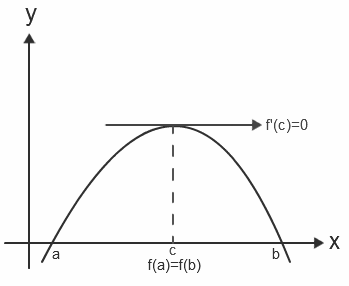
\includegraphics[width=0.6\textwidth]{RollesTheorem.png}
	\end{figure}
\end{theorem}
\begin{proof}[Proof of Rolle's Theorem]
	This theorem almost immediately follows from Theorem \ref{thm:extreme_value_theorem} and Theorem \ref{thm:max_derivative}. The only issue is that for Theorem \ref{thm:max_derivative} we need $a < c < b$ but the Extreme Value Theorem only guarantees $a \le c \le b$. So we need a small argument to fill this gap.

	By the Extremal Value Theorem, $f$ has an absolute maximum $c_{\max}$ and an absolute minimum $c_{\min}$ on the interval $[a,b]$.

	\begin{exercise}$ $
		\begin{enumerate}
			\item Argue that if $f(c_{\max}) = f(c_{\min})$ then $f$ is a constant function on $[a,b]$.
		\end{enumerate}
		We've already shown that for a constant function, $f'(x)$ equals 0, hence for every $c \in (a,b)$, $f'(c) = 0$ and we're done.

		So now we'll assume that $f(c_{\max}) \neq f(c_{\min})$.

		\begin{enumerate}[resume]
			\item 		Argue that in this case either $a < c_{\max} < b$ or $a < c_{\min}< b$ (possibly both).
			\item 		Finish the proof of Rolle's Theorem.
		\end{enumerate}
	\end{exercise}
\end{proof}

\begin{theorem}[Mean Value Theorem]
	Let $f$ be a differentiable function. For any interval $[a,b]$ there exists a real number $c \in (a,b)$ such that
	\begin{align*}
		f'(c) = \dfrac{f(b) - f(a)}{b - a}
	\end{align*}
	\begin{figure}[H]
		\centering
		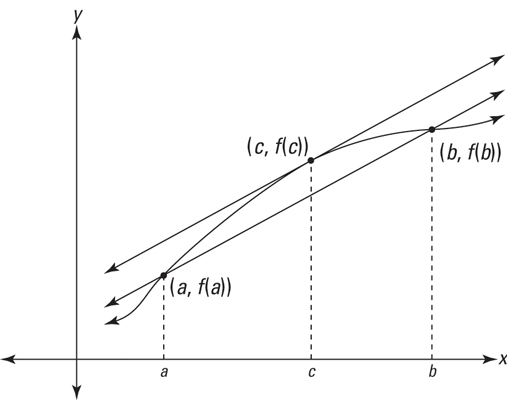
\includegraphics[width=0.6\textwidth]{MeanValueTheorem.jpg}
	\end{figure}
\end{theorem}
\begin{proof}[Proof of Mean Value Theorem]
	Mean Value Theorem follows from the Rolle's theorem by an algebraic trick.
	We'll construct a new function $g(x)$ that satisfies the hypotheses of Rolle's theorem.
	\begin{exercise}$ $
		\begin{enumerate}
			\item Find a real number $r$ such that $f(a) - r a = f(b) - r b$.
		\end{enumerate}
		For this value of $r$ define
		\begin{align*}
			g(x) = f(x) - r x
		\end{align*}
		By construction, $g$ is differentiable and satisfies $g(a) = g(b)$ and hence satisfies the hypotheses for Rolle's theorem. So, there exists some real number $ a < c < b$ such that
		\begin{align*}
			g'(c) = 0
		\end{align*}
		\begin{enumerate}[resume]
			\item Show that for this $c$, $f'(c) = \dfrac{f(b) - f(a)}{b - a}$, thereby completing the proof of Mean Value Theorem.
		\end{enumerate}
	\end{exercise}
\end{proof}

We'll see later on that the Mean Value Theorem is a key ingredient in the proof of Taylor series approximation. In fact, Taylor series approximations can be thought of as a generalization of MVT for higher order derivatives.




\subsection{L'Hopital's Rule}
We'll now (almost) provide a proof of L'Hopital's Rule using a stronger version of the Mean Value Theorem.
\begin{theorem}[Easy L'Hopital's Rule]
	Let $f$, $g$ be differentiable functions. Assume that
	\begin{align*}
		f(a) = 0 = g(a) \mbox{ \quad and \quad } g'(a) \neq 0,
	\end{align*}
	where $a$ is a real number. Then
	\begin{align*}
		\lim \limits_{x \rightarrow a} \dfrac{f(x)}{g(x)} = \dfrac{f'(a)}{g'(a)}
	\end{align*}
\end{theorem}
\begin{exercise}
	Notice that $\dfrac{f(x)}{g(x)} = \dfrac{f(x) - f(a)}{g(x) - g(a)}$. Use this to prove the easy version of L'Hopital's Rule. \hint{Divide the numerator and denominator by $x - a$ and take $\lim \limits_{x \rightarrow a}$.}
\end{exercise}

\begin{theorem}[Strong Mean Value Theorem]
	Let $f$, $g$ be differentiable functions. Assume that $g(a) \neq g(b)$ for some real numbers $a$ and $b$. Then there exists a real number $c \in (a,b)$ such that
	\begin{align*}
		\dfrac{f'(c)}{g'(c)} = \dfrac{f(b) - f(a)}{g(b) - g(a)}
	\end{align*}
\end{theorem}
\begin{proof}[Proof of Strong Mean Value Theorem]
	The Strong Mean Value Theorem follows from the Rolle's theorem by the same algebraic trick. We'll construct a new function $h(x)$ that satisfies the hypotheses of Rolle's theorem.
	\begin{exercise}$ $
		\begin{enumerate}
			\item Find a real number $r$ such that $f(a) - r g(a) = f(b) - r g(b)$.
		\end{enumerate}
		For this value of $r$ define
		\begin{align*}
			h(x) = f(x) - r g(x)
		\end{align*}
		By construction, $h$ is differentiable and satisfies $h(a) = h(b)$ and hence satisfies the hypotheses for Rolle's theorem. So, there exists some real number $ a < c < b$ such that
		\begin{align*}
			h'(c) = 0
		\end{align*}
		\begin{enumerate}[resume]
			\item Show that for this $c$, $\dfrac{f'(c)}{g'(c)} = \dfrac{f(b) - f(a)}{g(b) - g(a)}$, thereby completing the proof of the Strong Mean Value Theorem.
		\end{enumerate}
	\end{exercise}
\end{proof}

\begin{exercise}
	Explain how the Mean Value Theorem is a special case of the Strong Mean Value Theorem and how the Rolle's theorem is a special case of the Mean Value Theorem.
\end{exercise}
\begin{theorem}[L'Hopital's Rule]
	Let $f$, $g$ be differentiable functions. Assume that
	\begin{align*}
		f(a) = 0 = g(a)
	\end{align*}
	where $a$ is a real number. Then
	\begin{align*}
		\lim \limits_{x \rightarrow a} \dfrac{f(x)}{g(x)} = \lim \limits_{x \rightarrow a} \dfrac{f'(x)}{g'(x)}
	\end{align*}
\end{theorem}

\begin{proof}[Idea of the proof]
	For any $b$, by the Strong Mean Value Theorem, there exists a $c \in (a,b)$ such that
	\begin{align*}
		\dfrac{f'(c)}{g'(c)}          & = \dfrac{f(b) - f(a)}{g(b) - g(a)}                                \\
		\implies \dfrac{f'(c)}{g'(c)} & = \dfrac{f(b)}{g(b)}               & (\mbox{as } f(a) = 0 = g(a))
	\end{align*}
	As $c$ has to lie between $a$ and $b$, when we take the limit $b \rightarrow a$ we must also have $c \rightarrow a$. Taking limits of both sides we get the required result.
	\begin{align*}
		\lim \limits_{c \rightarrow a} \dfrac{f'(c)}{g'(c)} = \lim \limits_{b \rightarrow a}  \dfrac{f(b)}{g(b)}
	\end{align*}
\end{proof}

\begin{remark}
	The last argument in the above proof is not rigorous. While the idea is correct, to make it rigorous we need generalized notions of limits called {\bf limit superior} ($\lim \sup$) and {\bf limit inferior} ($\lim \inf$). This is unfortunately beyond the scope of this class.
\end{remark}

There are many more variants of L'Hopital's Rule: for one-sided limits, for $a = \infty$, for $ \lim \limits_{x \rightarrow a} f(a)= \infty =\lim \limits_{x \rightarrow a} g(a) $ etc. They can all be proven using similar techniques.










\subsection{First Derivative Test}
In this section, we'll prove the First Derivative Test for differentiable functions.

\begin{definition}
	We say that a function $f$ is {\bf increasing} on an interval $[a,b]$, if for all $x$, $y$ in $[a,b]$ if $x < y$ then $f(x) \le f(y)$.
		We say that $f$ is {\bf strictly increasing} on $[a,b]$, if for all $x$, $y$ in $[a,b]$ if $x < y$ then $f(x) < f(y)$.
\end{definition}
\begin{exercise}
	Come up with a definition for when a function is {\bf decreasing}, {\bf strictly decreasing} on an interval.
\end{exercise}
\begin{exercise}
	Find the interval(s) on which the function $x^2$ is increasing/decreasing? What about the function $x^3$?
\end{exercise}

For differentiable functions, we can determine if a function is increasing or decreasing by calculating it's first derivative.
\begin{exercise}$ $
	\label{q:increasing_decreasing_derivative}
	\begin{enumerate}
		\item {\bf Optional:} Let $g(x)$ be a function such that $\lim \limits_{x\rightarrow c} g(x)$ exists for some real number $c$ in the interval $(a,b)$. Prove that if $g(x) \ge 0$ for all $x$ in $[a,b]$, then $\lim \limits_{x\rightarrow c} g(x)$ is also $\ge 0$.\hint{Proof by Contradiction.}\\ {\it (You can assume this part to be true if you choose not to prove it.)}
		\item Let $f(x)$ be an increasing function on $[a,b]$ and let $c \in (a,b)$. Prove that $g(x) \ge 0$ on the interval $[a,b]$ where $g(x)$ is the function
		      \begin{align*}
			      g(x) = \dfrac{f(x) - f(c)}{x - c}
		      \end{align*}
		\item Let $f(x)$ be a differentiable function that is increasing on the interval $[a,b]$. Prove that all $c \in (a,b)$, $f'(c) \ge 0$. Similarly, for decreasing functions.
	\end{enumerate}
\end{exercise}
Note that this agrees with the interpretation of a derivative as the {\it instantaneous} rate of change of a function: an increasing function should have a positive {instantaneous} rate of change and a decreasing function should have a negative {instantaneous} rate of change. The converse of the above statement is almost true, but for this we need an extra assumption on $f$ and the proof is a bit more intricate.

\begin{prop}
	\label{thm:increasing_positive_derivative}
	If $f'(x) > 0$ for all $c \in (a,b)$ then $f$ is strictly increasing on $(a,b)$. Similarly, for $f'(c) < 0$.
\end{prop}

\begin{exercise}
	Let $f'(x) > 0$ for all $c \in (a,b)$. Prove by Contradiction, that for all $x$, $y \in (a,b)$, if $x < y$ then $f(x) < f(y)$.\hint{Use the Mean Value Theorem.}
\end{exercise}

\begin{exercise}
	Use the above Proposition to find the range in which the function $x^n$ is increasing/decreasing, where $n$ is a positive integer.
\end{exercise}

\begin{definition}A real number $c$ is said to be a {\bf local maximum} of a function $f$ if there is some interval $(a,b)$ containing $c$ such that if $a < x < b$ then $f(c) \ge f(x)$.
\end{definition}
\begin{exercise}
	Come up with a definition for {\bf local minimum}.
\end{exercise}
\begin{exercise} Assume that the function $f(x)$ is differentiable and it's derivative $f'(x)$ is continuous. Using Proposition \ref{thm:increasing_positive_derivative} prove that if $c$ is a local maximum of $f(x)$ then $f'(c) = 0$.\hint{Proof by Contradiction.} Similarly for a local minimum.
\end{exercise}
\begin{remark}
	We need $f'(x)$ to be continuous to ensure that if $f'(c) > 0$ then $f'(x) > 0$ for every $ x \in (a,b)$, where $(a,b)$ is some interval containing $c$.
\end{remark}



Combining everything in this section we have proven the following Theorem, also called the {\bf First Derivative Test}.
\begin{theorem}[First Derivative Test]
	Let $f(x)$ be a differentiable function whose derivative $f'(x)$ is a continuous function.

	For a real number $c$,
	\begin{align*}
		f	\mbox{ has a local max/min at } c & \implies f'(c) = 0   \\
		f \mbox{ is increasing near } c    & \implies f'(c) \ge 0 \\
		f \mbox{ is decreasing near } c    & \implies f'(c) \le 0
	\end{align*}
	Conversely,
	\begin{align*}
		f'(c) > 0 & \implies f \mbox{ is increasing near } c \\
		f'(c) < 0 & \implies f \mbox{ is decreasing near } c
	\end{align*}
	where by ``near $c$'' means for some interval $(a,b)$ containing $c$.
\end{theorem}

A real number $c$ satisfying $f'(c) = 0$ is called a {\bf critical point} of $f$. The First Derivative Test says that a local max/min has to be a critical point, but it does not say that a critical point has to be a local max/min. A standard example of this failure is $c=0$ for the function $f(x) = x^3$.
\begin{align*}
	\mbox{Local min/max}  & \Rightarrow \mbox{Critical point}    \\
	\mbox{Critical point} & \not\Rightarrow \mbox{Local min/max}
\end{align*}
There are ways to fix this using higher derivatives. We'll do this later using Taylor Series approximations.



\subsubsection*{Optional Problems}
There are multiple ways of proving Proposition \ref{thm:increasing_positive_derivative}. However, all the methods require some additional techniques which we have not yet developed.

\begin{exercise}
	Try to write down a rigorous proof of Proposition \ref{thm:increasing_positive_derivative}. What statement {\it should} be true for your proof to work?
\end{exercise}









\subsection{Convexity and Concavity}
The second derivative of a function $f(x)$ is defined as
\begin{align*}
	f''(x) = \left(f'(x)\right)'
\end{align*}
If the second derivative exists then we say that a function is {\bf twice differentiable}.
More generally, the $n^{th}$ derivative $f^{(n)}(x)$ is defined as
\begin{align*}
	f^{(n)}(x) = \left(f^{(n-1)}(x)\right)'
\end{align*} If all derivatives exist then we say that the function is {\bf smooth} or {\bf infinitely differentiable}. The standard functions like polynomials, trig functions, exponentials, and logarithms are all smooth wherever they're defined.\\

If a function $f$ is twice differentiable, then the second derivative of $f$ measures it's convexity/concavity.
\begin{definition}
	A function $f$ is said to be {\bf convex} (or {\bf concave upwards}) on an interval, if for every real numbers $a$, $b$ in the interval, the graph of $f(x)$ lies below the line joining $(a,f(a))$ to $(b,f(b))$.
	\begin{figure}[H]
		\centering
		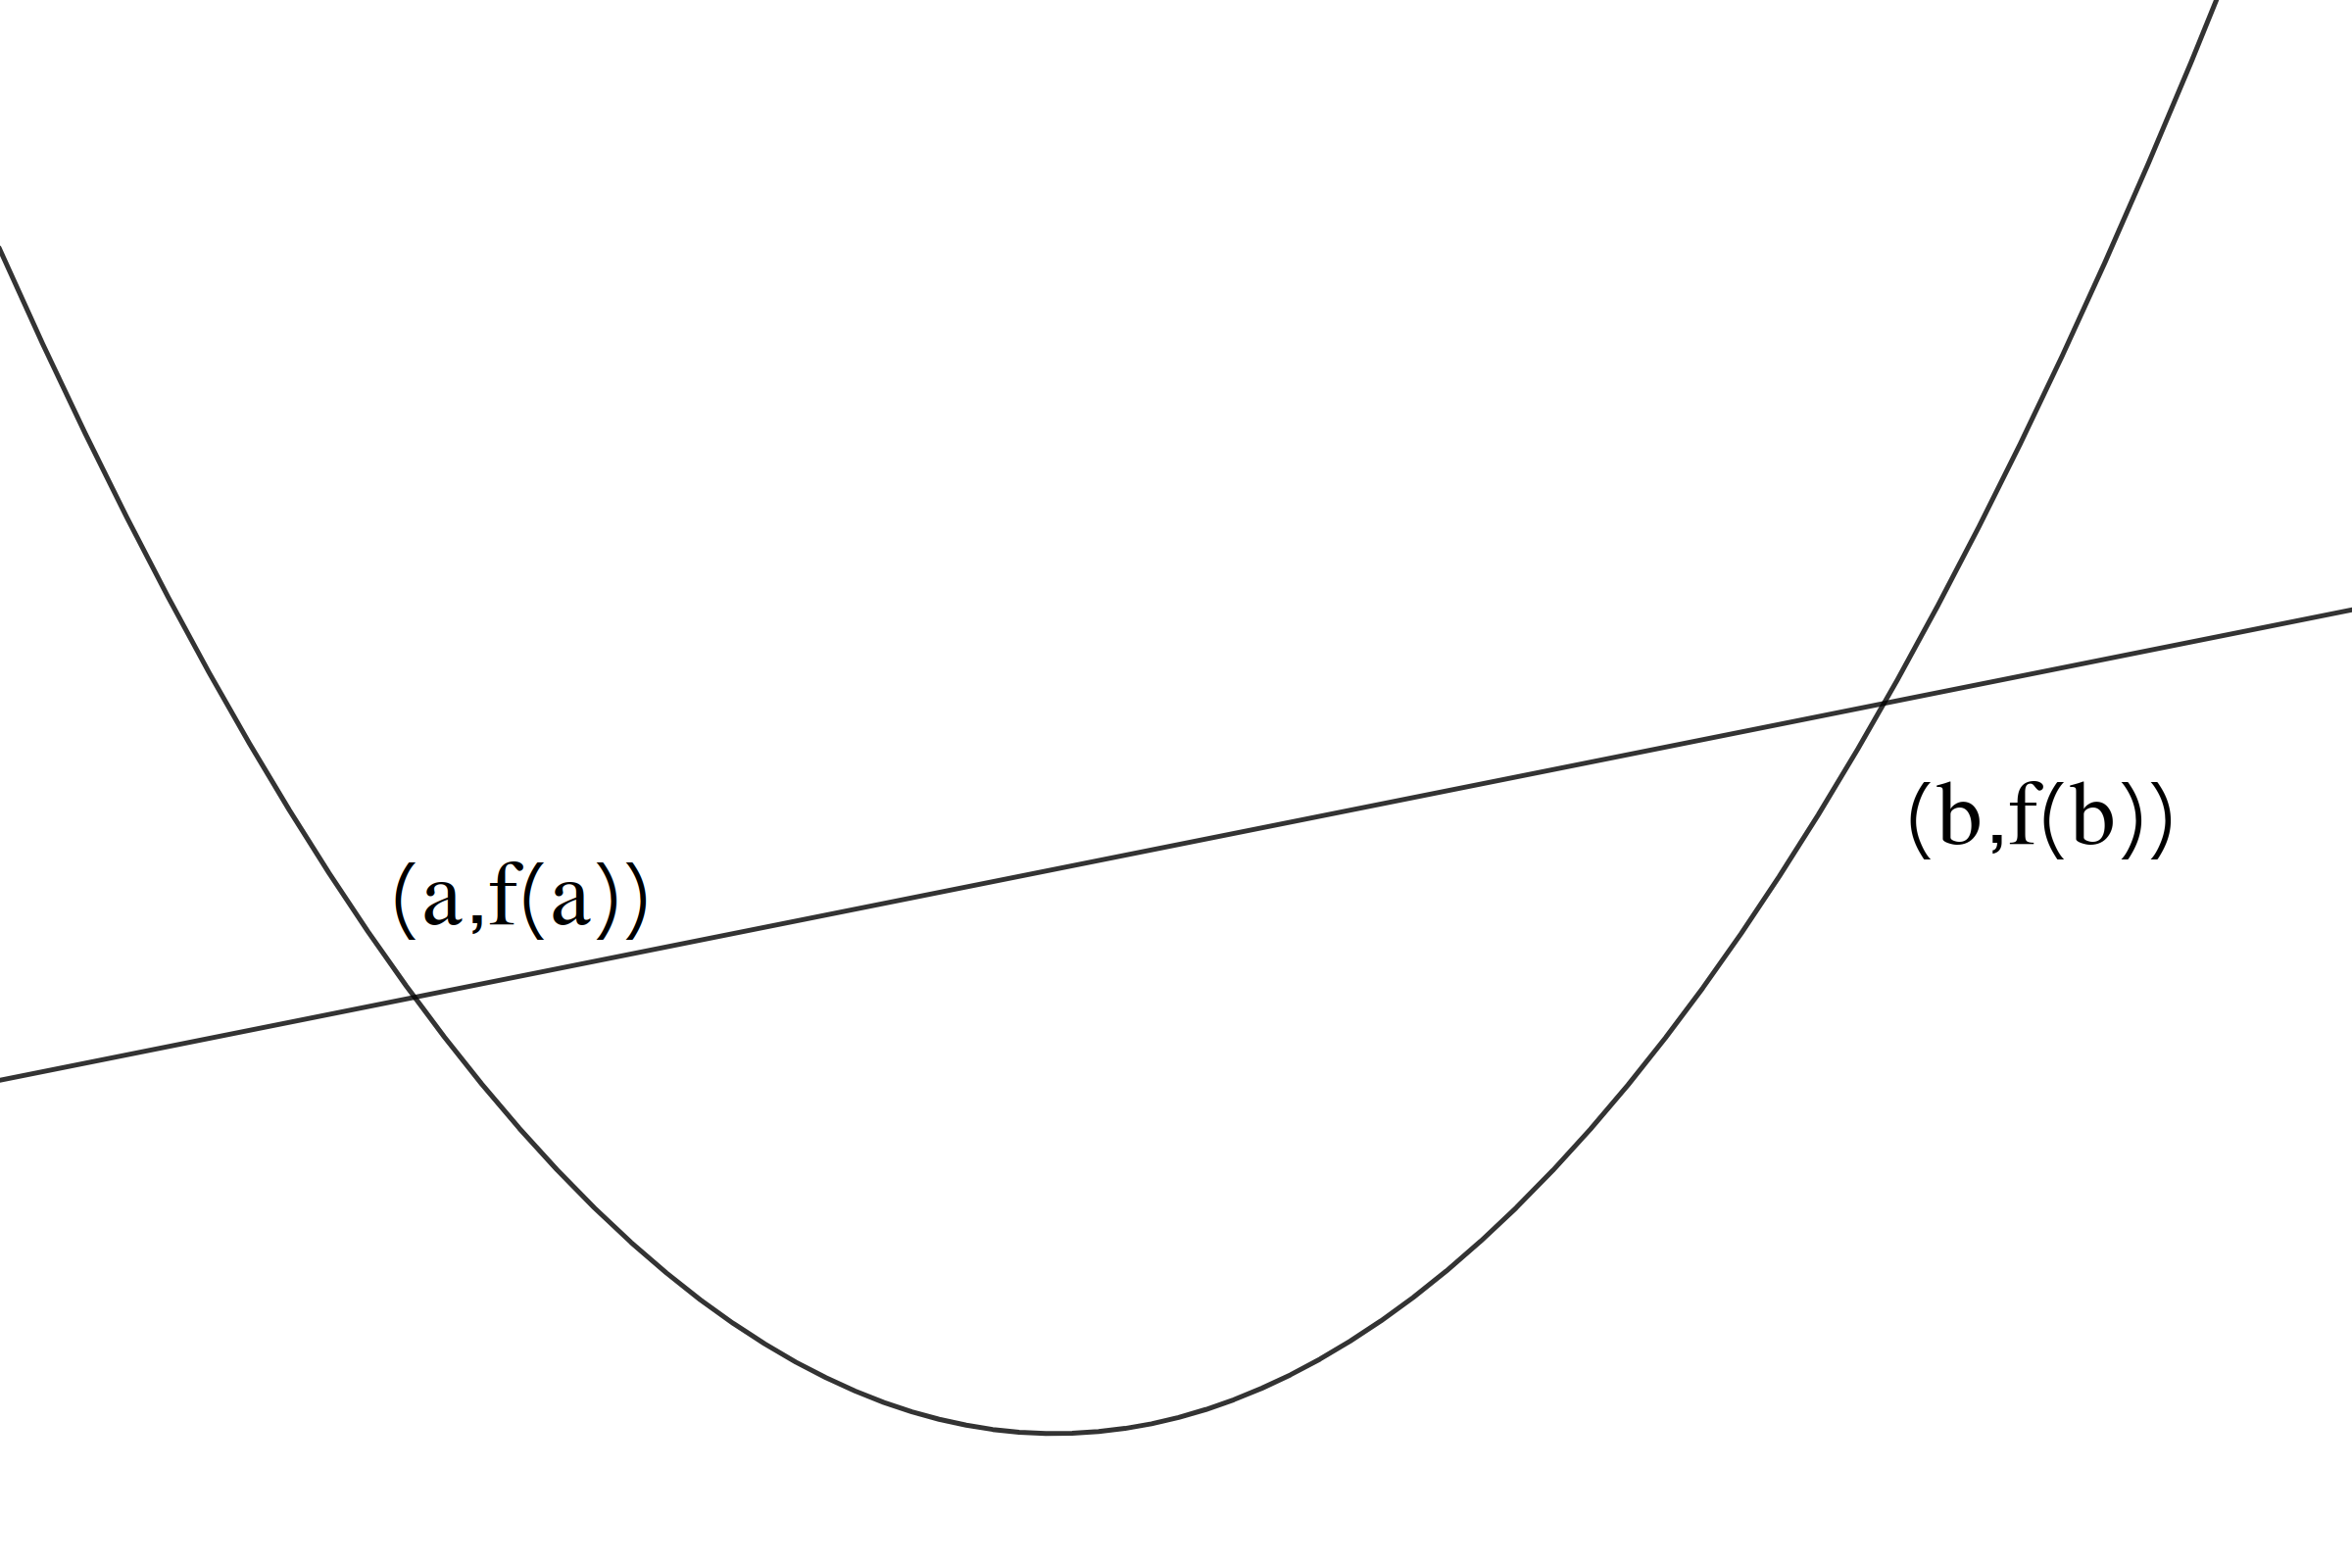
\includegraphics[width=0.6\textwidth]{ConvexFunction.png}
	\end{figure}
\end{definition}
Convex functions play an important role in many areas of mathematics, especially in the study of optimization problems.\\

The following theorem establishes the connection between convexity and the second derivative.
\begin{theorem}
	\label{thm:convex_functions}
	Let $f$ be a twice differential function.

	If $f$ is convex on an interval then $f''(x) \ge 0$ on that interval. Conversely, if for every real number $x$ in some interval, $f''(x) > 0$, then $f$ is convex on that interval.
\end{theorem}

\begin{remark}
	To avoid clutter, we'll often drop the terms {\it on an interval, in some interval} etc. in the following proof. Just keep in mind that there is an ambient interval and all our variables belong to that interval.
\end{remark}

\noindent \begin{tabular}{|p{\textwidth}|}
  \hline \\{\it Once you have solved all the exercises below, submit your final solutions as one single logically coherent proof. Also include all the text that is in between the exercises, so that you yourself see how all the pieces fit together. As before, this is to practice writing complex proofs.}\\\\
  \hline
\end{tabular}

\begin{proof}
	Let $f$ be a twice differential function.
	\begin{exercise}
		For real numbers $a$, $b$ denote by $m_{a,b}$ the slope of the line joining the points $(a,f(a))$ and $(b,f(b))$.
		Find a formula for $m_{a,b}$.
	\end{exercise}

	\noindent We'll first prove the forward direction.\\
	\noindent {\bf Claim:} {\it 	If $f$ is convex on an interval then $f''(x) \ge 0$ on that interval.}

	We'll prove that $f'(x)$ is an increasing function which will then imply that $f''(x) \ge 0$ (as the derivative of an increasing function is $\ge 0$).\\

	Let $f$ be a convex function. Let $a < b$ be two real numbers.
	\begin{exercise}
		Let $a < x < y$ be real numbers.
		\begin{enumerate}
			\item {\it Geometrically} argue that $m_{a,x} < m_{a,y}$.
			\begin{figure}[H]
				\centering
				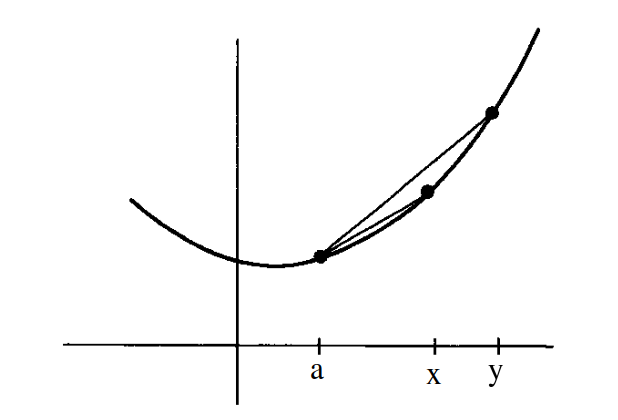
\includegraphics[width=0.6\textwidth]{ConvexFunctionProof1.png}
			\end{figure}
			\item Using the formula for $m_{a,x}$, $m_{a,y}$ and the above inequality argue that $$f'(a) \le m_{a,y}$$ for real numbers $a < y$.
		\end{enumerate}
	\end{exercise}

	\begin{exercise}
		Let $x < y < b$ be real numbers.
		\begin{enumerate}
			\item {\it Geometrically} argue that $m_{x,b} < m_{y,b}$.
			\item Using the formula for $m_{y,b}$, $m_{x,b}$ and the above inequality argue that $$m_{x,b} \le f'(b) $$ for real numbers $x < b$.
		\end{enumerate}
	\end{exercise}

	\begin{exercise}
		Combine the results from the previous two exercises to conclude that $f'(a) \le f'(b)$.
	\end{exercise}
	Hence $f'(x)$ is an increasing function and hence $f''(x) \ge 0$.\\

	\noindent We'll next prove the other direction. \\
	\noindent {\bf Claim:} {\it If for every real number $x$ in some interval, $f''(x) > 0$, then $f$ is convex on that interval.}

	We'll prove this by {\it contradiction}. Let $f$ be a function such that $f''(x) > 0$ on some interval. This implies that $f'(x)$ is an increasing function on that interval. This is the statement that we'll contradict.\\

	Assume on the contrary that $f$ is not convex. This means that for some real numbers $a < b$, there exists a number $c$ with $a < c < b$ such that the point $(c,f(c))$ lies above the line joining $(a,f(a))$ and $(b,f(b))$.

	\begin{exercise}
		Draw a picture.
	\end{exercise}
	Applying the Mean Value Theorem to the intervals $[a,c]$ and $[c,b]$ gives us real numbers $d_1 \in (a,c)$ and $d_2 \in (c,b)$ such that
	\begin{align*}
		f'(d_1) = m_{a,c} \mbox{ and } f'(d_2) = m_{c,b}
	\end{align*}

	\begin{exercise} $ $
		\begin{enumerate}
			\item Draw a picture.
			\item {\it Geometrically} argue that $f'(d_1) > f'(d_2)$.
			\item Why is this a contradiction?
		\end{enumerate}
	This completes a proof of the other direction, and hence of the main theorem.
	\end{exercise}
\end{proof}

\subsubsection{Second Derivative Test}
Let $f(x)$ be a twice differentiable function. If a real number $c$ is a local minimum of $f$ then $f$ is convex on some interval containing $c$. A similar statement is true when $c$ is a local maximum. Combining this observation with the previous Theorem and the First Derivative Test, we get the {\bf Second Derivative Test}.

\begin{theorem}[Second Derivative Test]
	Let $f(x)$ be a twice differentiable function whose second derivative $f''(x)$ is a continuous function.
	\begin{align*}
		f	\mbox{ has a local min at } c &\implies f'(c) = 0 \mbox{ and } f''(c) \ge 0 \\
			f	\mbox{ has a local max at } c &\implies f'(c) = 0 \mbox{ and } f''(c) \le 0
	\end{align*}
	Conversely,
	\begin{align*}
		f'(c) = 0 \mbox{ and } f''(c) > 0 & \implies f	\mbox{ has a local min at } c  \\
		f'(c) = 0 \mbox{ and } f''(c) < 0 & \implies f	\mbox{ has a local max at } c
	\end{align*}
\end{theorem}
We need continuity of $f''(x)$ so that $f''(c) > 0$ implies $f''(x)>0$ on some interval containing $c$.


\subsubsection*{Optional Problems}
\begin{exercise}$ $
	\begin{enumerate}
		\item Find an example of a function which is convex but $f''(x)$ is not always $> 0$.
		\item Why does the proof of Theorem \ref{thm:convex_functions} only proves  that {\it if $f$ is convex then $f''(x) \ge 0$} (instead of $f''(x) > 0$)?
	\end{enumerate}
\end{exercise}

\begin{exercise}
	Several times in this section we used {\it geometric} arguments. This is less preferable than algebraic arguments as geometric arguments are not rigorous and hence susceptible to being incorrect.
	\begin{enumerate}
		\item Convert the definition of a convex function into an algebraic equation involving inequalities.
		\item Use this equation to rigorously prove that, say, $m_{a,x} < m_{a,y}$ if $a < x < y$.
	\end{enumerate}
\end{exercise}

\begin{exercise}
	Let $f$ be a convex function on an interval containing the real numbers $a$, $b$. Show that for all $ t \in [0,1]$,
	\begin{align*}
		f(t a + (1-t) b) \le t f(a) + (1- t) f(b)
	\end{align*}
	This inequality is called {\bf Jensen's inequality} for convex functions.
\end{exercise}

  %!TEX root=ClassNotes.tex

\section{Integrals}
\subsection{Integrals as Areas}

\begin{figure}[H]
	\centering
	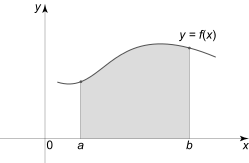
\includegraphics[width=0.5\textwidth]{integral.png}
	\caption*{Signed area under the curve is given by $\int_a^b f(t)\:dt$}
\end{figure}
The integral of a function captures the concept of an area.
\begin{align*}
	\int \limits_{a}^b f(t) dt = \mbox{ signed area between the curve $y=f(x)$ and the x-axis \strut}
\end{align*}
where by signed area we mean that the integral is negative if $f(x) < 0$ and hence equals negative of the area in this case (as area is always positive). This is a good {\it interpretation} but not a good {\it definition} as we have not rigorously defined what area is.
Instead we'll define the integral in terms of a limit and then define the (signed) area as the integral.

\begin{exercise}
	Express the following areas as (sums of) integrals. For each problem, draw pictures to justify your answer.
	\begin{enumerate}
		\item Area between the line $x + y = 1$, the x-axis and the y-axis.
		\item Area enclosed between the graph $y = \sin x$ and the x-axis for $x \in [0,2\pi]$.
		\item Area enclosed between the parabola $y=x^2$ and the line $y=1$.
		\item Area of a circle of radius 1.
	\end{enumerate}
\end{exercise}
Several physical quantities can be expressed as integrals, for example,
if $t$ denotes time and $f(t)$ is the speed of a particle then the integral measures the distance traveled, if $t$ denotes length and $f(t)$ is the linear density of a one dimensional object then the integral measures the total mass, etc.

\subsection{Definition of Integral}
We need several preliminary definitions to define the integral.
\begin{definition}$ $
	\begin{enumerate}
		\item For an interval $[a,b]$ a {\bf partition} $P$ is a sequence of real numbers
		      \begin{align*}
			      a = x_0 < x_1 < \dots < x_n = b
		      \end{align*}
		\item A {\bf uniform partition} $P_n$ of $[a,b]$ is the {\it uniform length} partition
		      \begin{align*}
			      x_0 & = a                          \\
			      x_1 & = a + \dfrac{b-a}{n}         \\
			          & \:\:\: \vdots                \\
			      x_i & = a + i \cdot \dfrac{b-a}{n} \\
			          & \:\:\: \vdots                \\
			      x_n & = b
		      \end{align*}
		\item For a partition $P$ define
		      \begin{align*}
			      M_i & = \sup \{ f(x) : x_i \le x \le x_{i+1}\} \\
			      m_i & = \inf \{ f(x) : x_i \le x \le x_{i+1}\}
		      \end{align*}
		      Define the {\bf upper Riemann sum} $U(f,P)$ and the {\bf lower Riemann sum} $L(f,P)$ as
		      \begin{align*}
			      U(f,P) & = \sum \limits_{i=0}^{n-1} M_i \cdot (x_{i+1} - x_i) \\
			      L(f,P) & = \sum \limits_{i=0}^{n-1} m_i \cdot (x_{i+1} - x_i)
		      \end{align*}
	\end{enumerate}
\end{definition}
\begin{figure}[H]
	\centering
	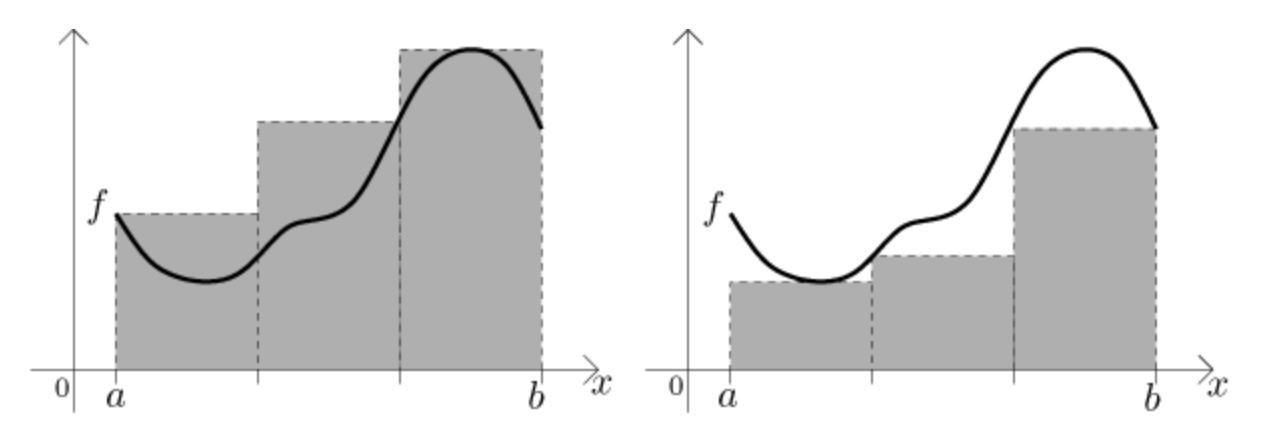
\includegraphics[width=0.8\textwidth]{RiemannSums2.png}
	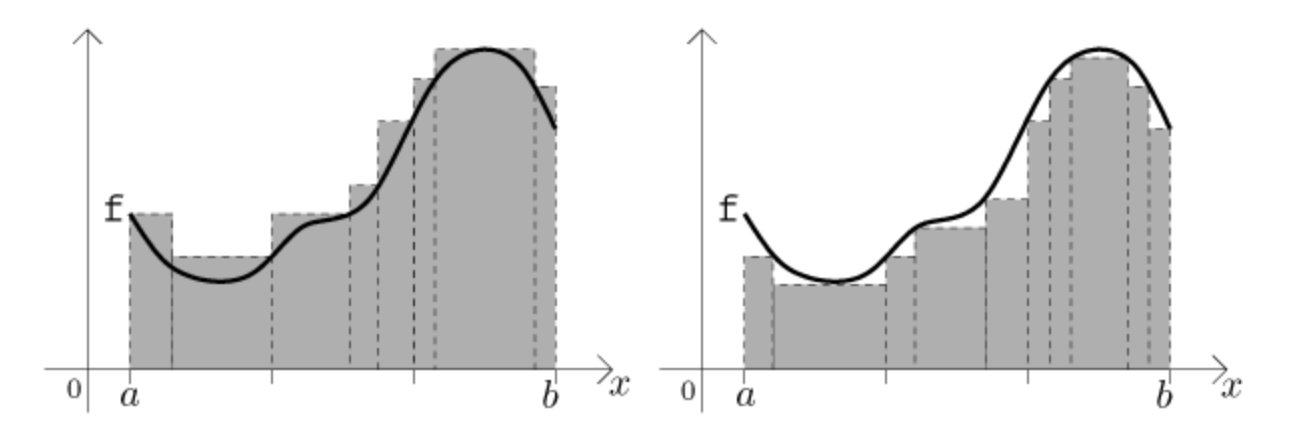
\includegraphics[width=0.8\textwidth]{RiemannSums1.png}
	\caption*{For finer partitions, the Riemann sums provide better approximations of the integral, hence in the limiting case as $n\rightarrow \infty$ we obtain the exact integral.}
\end{figure}
\begin{definition}
	\label{def:definition_Integral}
	We say that a function $f(x)$ is (Riemann) {\bf integrable} on an interval $[a,b]$ if there exists a real number $I$ such that
	\begin{align*}
		\lim \limits_{ n \rightarrow \infty} U(f,P_n) = I = \lim \limits_{ n \rightarrow \infty} L(f,P_n)
	\end{align*}
	In this case, we define the integral of $f$ on $[a,b]$ as
	\begin{align*}
		\int \limits_{a}^{b} f(t) \: dt & = I
	\end{align*}
\end{definition}
\noindent Thus when a function $f(x)$ is integrable it suffices to compute either $\lim \limits_{ n \rightarrow \infty} U(f,P_n)$ or $\lim \limits_{ n \rightarrow \infty} L(f,P_n)$ to compute the integral. \\

We'll assume the following theorem without proof. The proof requires the notion of {\bf uniform continuity} which is beyond the scope of this class.

\begin{theorem}
	\label{theorem:continuous_are_integrable}
	If $f$ is a continuous function on the interval $[a,b]$ then $f$ is integrable on $[a,b]$.
\end{theorem}

We'll do a few examples to better understand the definition of integral.
\begin{exercise}
	Let $f(x) = -x$, let $a=0$ and $b = 1$.
	\begin{enumerate}
		\item Use basic geometry to find $\int_{0}^1 f(t) \: dt$.
		\item Using pictures describe and compute $L(f,P_1)$, $L(f,P_2)$, and $L(f,P_3)$.
		\item Compute $L(f,P_n)$ where $n$ is a positive integer. You'll need to use
		      \begin{align*}
			      1 + 2 + 3 + \dots + n = \dfrac{n(n+1)}{2}
		      \end{align*}
		\item Find $\lim \limits_{n \rightarrow \infty} L(f,P_n)$, which equals $\int_{0}^1 f(t) \: dt$ by Theorem \ref{theorem:continuous_are_integrable}, and verify that it agrees with part 1.
	\end{enumerate}
\end{exercise}

\begin{exercise}
	Let $f(x) = x^2$, let $a=0$ and $b = 1$.
	\begin{enumerate}
		\item Compute $U(f,P_n)$ where $n$ is a positive integer. You'll need to use the identity
		      \begin{align*}
			      1^2 + 2^2 + 3^2 + \dots + n^2 = \dfrac{n(n+1)(2n+1)}{6}
		      \end{align*}
		\item Find $\lim \limits_{n \rightarrow \infty} U(f,P_n)$, which equals $\int_{0}^1 f(t) \: dt$ by Theorem \ref{theorem:continuous_are_integrable}.
	\end{enumerate}
\end{exercise}

\begin{exercise}
	Let $a = 0$, $b = 1$, and let
	\begin{align*}
		f(x) = \begin{cases}
			1 & \mbox{ if $x$ is rational}    \\
			0 & \mbox{ if $x$ is irrational.}
		\end{cases}
	\end{align*}
	\begin{enumerate}
		\item For $n$ a positive integer, compute $U(f,P_n)$ and $L(f,P_n)$.
		\item Find $\lim \limits_{n \rightarrow \infty} U(f,P_n)$ and $\lim \limits_{n \rightarrow \infty} L(f,P_n)$ and show that the $f(x)$ is not integrable.
	\end{enumerate}
\end{exercise}



\subsubsection{Indefinite Integrals}
We'll assume the following theorem without proof.
\begin{theorem}
	\label{theorem:integral_sum}
	For real numbers $a < b < c$, if $f$ is integrable on $[a,c]$ then
	\begin{align*}
		\int \limits_a ^c f(t) \: dt = \int \limits_a ^b f(t) \: dt  + \int \limits_b ^c f(t) \: dt
	\end{align*}
\end{theorem}
\begin{exercise}
	Draw a picture to explain the statement of the above theorem.
\end{exercise}

So far, we've only defined $\int_a^b f(t) \: dt$ for $a < b$. We now extend this to all real numbers $a$, $b$ by defining
\begin{align*}
	\int \limits_a^a f(t) \:dt
	= 0
	 &  & \mbox{ and } &  &
	\int \limits_a^b f(t) \:dt
	= -\int \limits_b^a f(t) \:dt
	\mbox{ \quad if } a > b
\end{align*}
With this extended notation one can check that Theorem \ref{theorem:integral_sum} is true for all real numbers $a$, $b$, $c$. For example, for $ a < b < c$
\begin{align*}
	         &  &
	\int \limits_a ^c f(t) \: dt = \int \limits_a ^b f(t) \: dt  + \int \limits_b ^c f(t) \: dt \\
	\implies &  &
	\int \limits_a ^c f(t) \: dt = \int \limits_a ^b f(t) \: dt  - \int \limits_c ^b f(t) \: dt \\
	\implies &  &
	\int \limits_a ^c f(t) \: dt + \int \limits_c ^b f(t) \: dt = \int \limits_a ^b f(t) \: dt
\end{align*}


\begin{definition}
	For an integrable function $f$ and a real number $a$, an {\bf antiderivative} is a function on the real numbers defined as
	\begin{align*}
		F_a(x) = \int \limits_a^x f(t) \: dt
	\end{align*}
\end{definition}

\begin{exercise}
	\label{q:difference_antiderivatives}
	For real numbers $a$, $b$ show that
	\begin{align*}
		F_a(x) - F_b(x)
	\end{align*}
	is a constant that does not depend on $x$.
\end{exercise}

Thus for any integrable function $f$ any two antiderivatives differ by a constant. This allows us to {\it define} the {\bf indefinite integral} denoted
\begin{align*}
	\int f(x) \: dx
\end{align*}
as $\int_a^x f(t) \: dt$ for some real number $a$. Changing the constant $a$ changes $F_a(x)$ by a constant, hence the indefinite integral is only defined up to a constant.

  %!TEX root=ClassNotes.tex
\section{Fundamental Theorem of Calculus}

The Fundamental Theorem of Calculus is a remarkable theorem that connects the notions of derivatives and integrals.

If we denote by $\mathcal{D}$ the {\it operator} that takes a function and produces it's derivative i.e. $\mathcal{D}(f) = f'$ and by $\mathcal{I}$ the {\it operator} that takes a function and produces (one of) it's antiderivative i.e. $\mathcal{I}(f) = \int_a^x f(t) \: \:dt$, for some real number $a$, then the Fundamental Theorem of Calculus says that
\begin{enumerate}
	\item $\mathcal{D}(\mathcal{I}(f)) = f$, and
	\item  $\mathcal{I}(\mathcal{D}(f)) = f + $ a constant.
\end{enumerate} so that Integral and Derivative are (almost) inverse operators.\footnote{Compare this to the definition of inverse functions: $f(g(x)) = x$ and $g(f(x)) = x$.} This is why $\int_a^x f(t) \: \:dt$ is called (an) {antiderivative}.\\



\begin{theorem}[Fundamental Theorem of Calculus]$ $
	\begin{description}
		\item[Form 1] Let $f$ be a continuous function. For a real number $a$, let $ F_a(x) = \int \limits_a^x f(t) \:dt$.
		      Then $F_a(x)$ is differentiable with
		      \begin{align*}
			      F_a'(x) = f(x).
		      \end{align*}
		\item[Form 2]
		      Let $f$ be a differentiable function with $f'$ continuous. Then for any real numbers $a$ and $x$,
		      \begin{align*}
			      \int \limits_a^x f'(t) \:dt = f(x) - f(a).
		      \end{align*}
	\end{description}
\end{theorem}

The idea of the proof of Form 1 is very straightforward. By definition of derivative,
\begin{align}
	\begin{split}
		F_a'(x)
		& = \lim \limits_{h \rightarrow 0} \dfrac{F_a(x+h) - F_a(x)}{h}                                                                                                 \\
		& = \lim \limits_{h \rightarrow 0} \dfrac{\int \limits_a^{x+h} f(t) \:dt - \int \limits_a^x f(t) \:dt}{h}                                                           \\
		& = \lim \limits_{h \rightarrow 0} \dfrac{\int \limits_x^{x+h} f(t) \:dt}{h}
		\qquad
		\qquad
		\mbox{ by Exercise } \ref{q:difference_antiderivatives}
	\end{split}
	\label{eq:Fundamental_Theorem_Reduction}
\end{align}
For small $h$ this last integral can be approximated by the area of a rectangle with height $f(x)$ and base $h$.
\begin{align*}
	\int \limits_x^{x+h} f(t) \:dt
	 & \approx f(x) \cdot h \\
	\implies \dfrac{\int \limits_x^{x+h} f(t) \:dt}{h}
	 & \approx f(x)
\end{align*}
We'll make this last statement precise using $\epsilon, \delta$ arguments. We'll start with a small Proposition.
\begin{figure}[t]
	\centering
	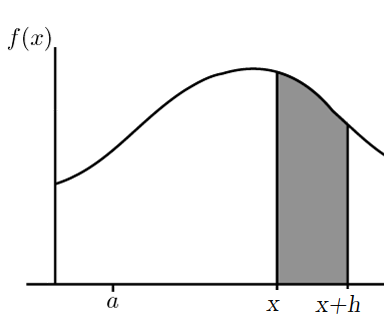
\includegraphics[width=0.6\textwidth]{FundamentalTheorem.png}
	\caption*{The area $\int_x^{x+h} f(t)\:dt$ can be approximated by a rectangle with height $f(x)$ and base $h$.}
\end{figure}

\begin{prop}
	\label{theorem:Fundamental_theorem_lemma}
	If for all $ y$ in the interval $(x,x+h)$,
	\begin{align*}
	m < f(y) < M
	\end{align*}
	for some real numbers $m$, $M$, then
	\begin{align*}
		mh < \int \limits_{a}^{b} f(t) \: \:dt < Mh
	\end{align*}
\end{prop}
\begin{exercise}$ $
	\begin{enumerate}
		\item Prove the above Proposition using a {\it geometric} argument.
		\item \textbf{Optional: } Prove the above Proposition rigorously using the definition of integral involving Riemann sums.
	\end{enumerate}
\end{exercise}

Now we get back to the proof of the Form 1 of the Fundamental Theorem of Calculus.
\begin{proof}[Proof of Form 1 of the Fundamental Theorem of Calculus]
	Let $f(x)$ be a continuous function, let $a$ be a real number. We want to show that
	\begin{align*}
		F_a'(x) = f(x)
	\end{align*}
	By Equations \eqref{eq:Fundamental_Theorem_Reduction} this is equivalent to proving that
	\begin{align*}
		\lim \limits_{h \rightarrow 0}\dfrac{\int \limits_x^{x+h} f(t) \:dt}{h}
		 & = f(x)
	\end{align*}
	We'll only prove this for the right hand limit, the left hand limit is proved similarly. We want to show that
	\begin{align}
		\label{eq:Fundamental_theorem_limit}
		\lim \limits_{h \rightarrow 0^+}\dfrac{\int \limits_x^{x+h} f(t) \:dt}{h}
		 & = f(x)
	\end{align}
	\begin{exercise}
		\label{q:epsilon_delta_limit}
		Convert Equation \eqref{eq:Fundamental_theorem_limit} into an $\epsilon, \delta$ statement using the definition of limit.
	\end{exercise}

	\begin{exercise}
		Recall what it means for $f(x)$ to be continuous from the right, using the  $\epsilon, \delta$ definition of continuity.
	\end{exercise}

	\begin{exercise}
		Using this $\delta$ and Proposition \ref{theorem:Fundamental_theorem_lemma} prove the statement in Exercise \ref{q:epsilon_delta_limit}, thereby completing the proof of the Fundamental Theorem of Calculus.
	\end{exercise}
\end{proof}

\begin{exercise}[{\bf Optional}]
	Prove that $\lim \limits_{h \rightarrow 0^-}\dfrac{\int \limits_x^{x+h} f(t) \:dt}{h}
	= f(x)$. (Be careful of the signs.)
\end{exercise}


The Form 2 of the fundamental theorem follows directly from Form 1 using a small Proposition about derivatives.
\begin{prop}
	\label{theorem:Fundamental_theorem_lemma2}
	If $g(x)$ is a differentiable function such that $g'(x) = 0$ for all real numbers $x$, then $g(x)$ is a constant function i.e. $g(x) = g(y)$ for all real numbers $x$, $y$.
\end{prop}
\begin{exercise}
	Prove the above Proposition by Contradiction\hint{Use the Mean Value Theorem}.
\end{exercise}

\begin{proof}[Proof of Form 2 of the Fundamental Theorem of Calculus]
	Let $f$ be a diffentiable function with $f'$ continuous, and let $a$ be a real number. We want to show that
	\begin{align*}
		\int \limits_a^x f'(t) \:dt = f(x) - f(a)
	\end{align*}
	Consider the function
	\begin{align*}
		g(x) = f(x) - \int \limits_a^x f'(t) \:dt.
	\end{align*}
	\begin{exercise}
		Using Form 1 of the Fundamental Theorem and Proposition \ref{theorem:Fundamental_theorem_lemma2} prove that $g(x)$ is a constant function.
	\end{exercise}
	\begin{exercise}
		As $g$ is a constant function, for all real numbers $x$, $g(x) = g(a)$. Use this to prove Form 2 of the Fundamental Theorem of Calculus.
	\end{exercise}
\end{proof}

\begin{remark}
	For real numbers $b$, $c$,
		\begin{align*}
			\int \limits_b^c f(t) \:dt
			&= \int \limits_b^a f(t) \:dt + \int \limits_a^c f(t) \:dt\\
			&= -\int \limits_a^b f(t) \:dt + \int \limits_a^c f(t) \:dt\\
			&= F_a(c) - F_a(b)
		\end{align*}
	where $F_a(x)$ is {\it an} antiderivative of $f(x)$ i.e. it is a function whose derivative is $f(x)$. This is the form is which the Fundamental Theorem of Calculus is most often used. Which $a$ we use to find the antiderivative does not matter, so the integral can be written in the following forms.
	\begin{align*}
		\int \limits_b^c f(t) \: \:dt
		&= F_a(c) - F_a(b) \\
		&= \left. F_a(x) \right|_{b}^c \\
		&= \left. \int f(x) dx \right|_{b}^c \\
		&= \left. \int f(x) dx \right|_{x=b}^{x=c}
	\end{align*}
	It is acceptable to use any of these forms as they all mean the same thing.
\end{remark}

\newpage
\subsection{Understanding the Fundamental Theorem of Calculus}
The Fundamental Theorem has a LOT of applications. We'll spend the next several sections just understanding this theorem.
\begin{exercise}
	Let $a$ be a real number. Find derivatives of the following functions using the Fundamental Theorem and simple algebraic manipulations.
	\begin{enumerate}
		\item $\int \limits_{x}^{a} f(t) \: dt$.
		\item $\int \limits_a^{x^2} f(t) \: dt$.
		\item $\int \limits_a^{g(x)} f(t) \: dt$, where	$g(x)$ is a differentiable function.
		\item $\int \limits_{x}^{x^2} f(t) \: dt$.
		\item $\int \limits_{h(x)}^{g(x)} f(t) \: dt$, where	$g(x)$, $h(x)$ are differentiable functions.
		% \item $\int \limits_a^{x} t \cdot f(t) \: dt$.
		\item $\int \limits_a^{x} x \cdot f(t) \: dt$. (Be careful!)
	\end{enumerate}
\end{exercise}

\begin{exercise}
	Prove that if
	\begin{align*}
		f'(t) > 0
	\end{align*}
	for all $t \in [a,b]$, then $f$ is increasing on the interval $[a,b]$ i.e. for all $x$, $y$ in the interval $[a,b]$ if $x < y$ then $f(x) < f(y)$.\hint{Compute the integral $\int \limits_x^y f'(t) \: dt$.}
\end{exercise}

\begin{theorem}[u-substitution]
	Let $f$, $g$ be differentiable functions. Then,
	\begin{align*}
		\int_a^x f(g(t)) g'(t)\: dt = \int_{g(a)}^{g(x)} f(u) \: du
	\end{align*}
\end{theorem}
\begin{exercise}[Proof of u-substitution] Consider the function
	\begin{align*}
		h(x)
		=
		\int_a^x f(g(t)) g'(t)\: dt - \int_{g(a)}^{g(x)} f(u) \: du
	\end{align*}
\begin{enumerate}
	\item Show that $h'(x) = 0$.
	\item Show that $h(a) = 0$.
	\item Argue that these two statements imply that $h(x) = 0$ for all $x$, thereby proving u-substitution.
\end{enumerate}
\end{exercise}


\begin{theorem}[Integration by parts]
	Let $f$, $g$ be differentiable functions. Then,
	\begin{align}
		\label{eq:integration_by_parts}
		\int_a^x f(t) g'(t)\: dt = f(x)g(x) - \int_{a}^{x} f'(t) g(t) \: dt + c
	\end{align}
	for some constant $c$.
\end{theorem}
\begin{exercise}[Proof of Integration by parts] Consider the function
	\begin{align*}
		h(x)
		=
		\int_a^x f(t) g'(t)\: dt - \left(f(x)g(x) - \int_{a}^{x} f'(t) g(t) \: dt \right)
	\end{align*}
Show that $h'(x) = 0$. Argue that this proves Integration by parts.
\end{exercise}

\begin{exercise}
	Find the contant $c$ in Equation \eqref{eq:integration_by_parts}.
\end{exercise}

Because of the constant $c$ that shows up in Equation \eqref{eq:integration_by_parts} integration by parts is often expressed using indefinite integrals as,
\begin{align*}
	\int f(x) g'(x)\: dx = f(x)g(x) - \int f'(x) g(x) \: dx + c
\end{align*}

\begin{remark}
	These two theorems
	\begin{itemize}
		\item u-substitution
		\item integration by parts
	\end{itemize}
	provide the main techniques for computing integrals. In the later sections we'll do several problems to practice these.
\end{remark}

  %!TEX root=ClassNotes.tex
\section{Trig, Exp, and Log functions}
We'll use the Fundamental Theorem of Calculus to compute the derivatives of trigonometric functions, exponentials, and logarithms.
\subsection{Trigonometric Functions}
In this section, we'll prove that
\begin{align*}
	(\cos x)' &= -\sin x\\
	(\sin x)' &= \cos x
	\end{align*}
We'll only show this for $0 < x < \pi/2$, however,  the statements are true for all real numbers $x$.
We'll do this by first computing $\left(\cos^{-1}x \right)'$ using basic geometry and the Fundamental Theorem and then using the formula for the derivative of inverse functions.

\begin{exercise}
	Consider the unit circle $x^2 + y^2 = 1$. In the following figure, the shaded region is a sector of angle $\theta$ (in radians), for $0 < \theta < \pi/2$, so that the corresponding point on the circle is $(\cos \theta, \sin \theta)$.
	\begin{align*}
		\adjincludegraphics[width=0.3\textwidth, valign=c]{pie1.png}
		=
		\adjincludegraphics[width=0.3\textwidth, valign=c]{pie2.png}
		+
		\adjincludegraphics[width=0.3\textwidth, valign=c]{pie3.png}
	\end{align*}
	\begin{enumerate}
		\item Argue that the above decomposition of areas can be expressed algebraically as
		      \begin{align*}
			      \dfrac{\theta}{2}
			       & =
			      \dfrac{x \sqrt{1 - x^2}}{2}
			      +
			      \int \limits_x^1 \sqrt{1 - t^2} \: dt
		      \end{align*}
		      which can further be simplified to
		      \begin{align*}
			      \dfrac{\cos^{-1}x}{2}
			       & =
			      \dfrac{x \sqrt{1 - x^2}}{2}
			      +
			      \int \limits_x^1 \sqrt{1 - t^2} \: dt
		      \end{align*}

		\item Differentiate both sides to show that
		      \begin{align*}
			      \left(\cos^{-1}x \right)'
			       & =
			      -\dfrac{1}{\sqrt{1-x^2}}
		      \end{align*}

		\item Use the formula for the derivative of inverse function\footnote{$\left(f^{-1}(a)\right)'= \dfrac{1}{f'(f^{-1}(a))}$} to show that
		      \begin{align*}
			      (\cos \theta)' = -\sin \theta
		      \end{align*}
	\end{enumerate}
\end{exercise}


\begin{exercise}
	Differentiate both sides of the trig identity
	\begin{align*}
		\sin^2 x  + \cos^2 x = 1
	\end{align*}
	and use your computation of $(\cos x)'$ to show that
	\begin{align*}
		(\sin x)' = \cos x
	\end{align*}
\end{exercise}

\begin{exercise}
	\begin{enumerate}
		\item Use the formula for the derivative of inverse function to compute the derivative of $\sin ^{-1}x$.
		\item What is the relationship between the derivatives of $\sin ^{-1}x$ and $\cos ^{-1}x$? Why do you think this is the case?
	\end{enumerate}
\end{exercise}

\begin{exercise}
	Compute the derivatives of $\tan x$ and $\tan^{-1} x$.
\end{exercise}


\subsection{Exponential Functions and Logarithms}
Exponential functions are a bit tricky to define from first principles as every natural definition of $e^x$ uses either limits of sequences or differential equations.
We'll instead give a more {\it ad hoc} definition of logarithms as in the book and {\it verify} that it satisfies the properties that logarithms are supposed to satisfy.

\begin{definition}
	Define the {\bf natural logarithm} to be the integral
		\begin{align*}
			\ln x = \int_1^x \dfrac{1}{t} \: dt
		\end{align*}
		for $x > 0$.
\end{definition}
\begin{remark}
	As $\ln x$ is {\it defined} to be the antiderivative of $ 1 / x$,
	\begin{align*}
		\left(\ln x\right)'= \dfrac{1}{x}
	\end{align*}
\end{remark}
\begin{exercise}
	\begin{enumerate}
		\item Draw the graph of $\dfrac{1}{x}$ for $x > 0$.
		\item {\it Geometrically} argue that
			\begin{align*}
				\ln x \mbox{ is }
				\begin{cases}
					\mbox{positive } & \mbox{ if } x > 1\\
					0 & \mbox{ if } x = 1\\
						\mbox{negative } & \mbox{ if } x < 1
				\end{cases}
			\end{align*}
		\item Using u-substitution\hint{In the u-substitution formula $
		\int_a^z f(g(t)) g'(t)\: dt = \int_{g(a)}^{g(z)} f(u) \: du$ use $g(t) = x \cdot t$.} show that
		\begin{align*}
			\int_1^y \dfrac{1}{t} \: dt
			&=
			\int_x^{xy} \dfrac{1}{t} \: dt
		\end{align*}
		for real numbers $x , y > 0$. (You should think about what this means geometrically.)
		\item Show that this implies that
		\begin{align}
			\label{eq:log_identity}
			\ln x + \ln y = \ln xy
		\end{align}
	\end{enumerate}
\end{exercise}
This last identity \eqref{eq:log_identity} is the fundamental identity of logarithms.

\begin{definition}
	Define $\exp(x)$ to be the inverse function of $\ln x$ i.e.
	\begin{align*}
		\exp(\ln x) &= x \\
		\ln(\exp x) &= x.
	\end{align*}
\end{definition}
\begin{definition}
	Define $e$ to be the value of $\exp(x)$ at $x = 1$.
\end{definition}


\begin{exercise}
	\begin{enumerate}
		\item Show that $\exp(0) = 1$.
		\item Show that Equation \eqref{eq:log_identity} implies that
		\begin{align*}
			\exp(a + b) = \exp(a) \cdot \exp(b)
		\end{align*}
		\item Use this to argue that
		\begin{align*}
			\exp(n) = e^n
		\end{align*}
		where $n$ is a positive integer.
		\item {\bf (Optional)} Extend the above statement first to negative integers and then to rational numbers.
	\end{enumerate}
	It follows then from continuity arguments that
	\begin{align*}
		\exp(x) = e^x
	\end{align*}
	for all real numbers $x$.
\end{exercise}


\begin{exercise}
	Use the formula for the derivative of inverse function to show that
	\begin{align*}
		\left(e^x\right)'=e^x\\
	\end{align*}
\end{exercise}



This completes the computation of derivatives of all the standard functions.

\begin{exercise}
	The Fundamental Theorem of Calculus says that if $f'(x)=g(x)$ then $f(x) = \int g(x)\: dx + c $, where $\int g(x)\: dx$ stands for the indefinite integral.
	Go back to your derivative computations in this section and rewrite them as indefinite integrals.
\end{exercise}

We'll next use the u-substitution, and Integration by Parts to compute integrals of functions which can be written in terms of these standard functions.














\newpage
\subsection{Trigonometric Identities}
We'll need several trigonometric identities for computing integrals.
While it is possible to derive these identities using Euclidean geometry, there is a much faster trick to derive these using {\it Euler's identity}.


\subsubsection{Complex Numbers}
First we need some basic algebraic facts about complex numbers. {\bf Complex numbers} are numbers of the form
\begin{align*}
	z = a + b i
\end{align*}
where $a$ and $b$ are real numbers and $i$ is a {\it formal} variable that satisfies
\begin{align*}
	i^2 = -1.
\end{align*} The number $a$ is called the {\bf real part} of $z$, denoted $\mathrm{Re}(z)$, and the number $b$ is called it's {\bf imaginary part}, denoted $\mathrm{Im}(z)$.

A real number $r$ can be thought of the complex number $ r + 0 i$. Thus the set of complex numbers contains the set of real numbers.

As with real numbers, we can add, subtract, multiply, and
divide complex numbers.
\begin{example} Multiplying complex numbers:
	\begin{align*}
			(a + bi)(c - di)
			&= a(c - di) + bi(c - di) \\
			&= ac - adi + bci + bd  & \mbox{ as } i^2 = -1\\
			&= (ac + bd) + i(-ad + bc)
	\end{align*}
\end{example}

\begin{exercise}
	\label{q:complex_conjugate}
	Show that
	\begin{align*}
		(a + bi) (a - bi) = a^2 + b^2.
	\end{align*}
\end{exercise}

The complex number $\overline{z} = a - bi$ is called the {\bf complex conjugate} of $z=a + bi$.
By the above exercise, we get a real number after multiplying a complex number by it's conjugate which is an extremely useful fact.

\begin{example}
		Complex conjugates are useful when dividing complex numbers. To simplify a fraction, we multiply and divide by the complex conjugate of the denominator.
		\begin{align*}
			\dfrac{a+bi}{c+di}
			&=
			\dfrac{a+bi}{c+di} \cdot	\dfrac{c - di}{c-di}\\
			&=
			\dfrac{(a+bi)(c - di)}{c^2+d^2} & \mbox{ by Exercise \eqref{q:complex_conjugate}}\\\
			&=
			\dfrac{(ac + bd) + i(-ad + bc)}{c^2+d^2} \\
			&=
			\dfrac{ac + bd}{c^2+d^2}
			+
			i\cdot \dfrac{-ad + bc}{c^2+d^2}
		\end{align*}
\end{example}

\begin{exercise}
	Find the real and imaginary parts of the following complex numbers:
	\begin{multicols}{2}
		\begin{enumerate}
			\item $(2-3i)(i)$
				\item $(2-3i)(1+i)$
					\item $\dfrac{1}{i}$
						\item $\dfrac{1}{1+i}$
							\item $\dfrac{2-3i}{i}$
								\item $\dfrac{2-3i}{1+i}$
		\end{enumerate}
	\end{multicols}
\end{exercise}



\subsubsection{Euler's Identity}
It is possible to extend trigonometric and exponential functions (but not logarithms) to complex numbers.
These functions have the same derivatives and integrals as in the real case.
The following {\bf Euler's Identity} establishes a deep connection between trigonometric and exponential functions.
\begin{theorem}[Euler's identity]
\begin{align*}
		e^{i \theta} = \cos \theta + i \sin \theta
\end{align*}
for all real numbers $\theta$.
\end{theorem}
The proof of this theorem requires us to extend the entire theory of calculus to complex numbers (called complex analysis) and is beyond the scope of this class.
We'll simply use it as a fast method of (re)deriving several trig identities, and later on for doing integrals computations.

\begin{example}
	We know that
	\begin{align*}
		&& e^{i \theta} \cdot e^{-i \theta} &= e^0
	\end{align*}
	Simplifying the left hand side we get,
	\begin{align*}
		\Rightarrow
		&&
		(\cos \theta + i \sin \theta) \cdot (\cos (-\theta) + i \sin (-\theta)) &= e^0  \\
		\Rightarrow
		&&
		(\cos \theta + i \sin \theta) \cdot (\cos \theta - i \sin \theta) &= 1  \\
		\Rightarrow &&
		\cos^2 \theta + \sin^2 \theta
		&= 1 & \mbox{ by \eqref{q:complex_conjugate}}
	\end{align*}
	which is the fundamental identity of trigonometric functions.
	(In the above derivation we used the fact that $\cos(-\theta) = \cos \theta$ and $\sin (-\theta) = - \sin \theta$.)
\end{example}

\begin{exercise}
	Using Euler's identity and
	\begin{align*}
		\left(e^{i \theta}\right)^2 = e^{2i \theta}
	\end{align*}
	find the formulae for $\cos 2 \theta$ and $\sin 2 \theta$. (These are called the {\bf double angle formulae}.)
\end{exercise}

\begin{exercise}
	\begin{enumerate}
		\item
		Using Euler's identity and
		\begin{align*}
			e^{i x} \cdot e^{i y}  = e^{i (x + y)}
		\end{align*}
		find the formulae for $\cos (x + y)$ and $\sin (x + y)$.
		\item
		Using Euler's identity and
		\begin{align*}
			e^{i x} \cdot e^{-i y}  = e^{i (x - y)}
		\end{align*}
		find the formulae for $\cos (x - y)$ and $\sin (x - y)$.
	\end{enumerate}
\end{exercise}


\begin{exercise}
	Using the previous exercise, show that
 \begin{align*}
		 2 \cos x \cos y &= \cos (x-y) + \cos(x+y) \\
	 2 \sin x \sin y &= \cos (x-y) - \cos(x+y)\\
		2 \sin x \cos y &= \sin (x-y) + \sin(x+y)
 \end{align*}
\end{exercise}

We'll now apply these identities to compute some definite integrals.
In later sections, we'll use these to compute indefinite integrals  such as $\int e^{ax} \sin {bx} \: dx$.

\begin{exercise}
	Let $n$ be an integer.
	\begin{enumerate}
		\item Draw graphs of
		\begin{align*}
			\sin x, \sin (-x), \sin 2x, \sin (-2x), \\
			\cos x, \cos (-x), \cos 2x, \cos (-2x),
		\end{align*} for $ -\pi \le x \le \pi$.
		\item Geometrically argue that
		\begin{align*}
			\int_{-\pi}^{\pi} \cos (nt) \: dt &=
			\begin{cases}
				0 & \mbox{ if } n \neq 0 \\
				2 \pi & \mbox{ if } n = 0
			\end{cases}
		\end{align*}
		\item Geometrically argue that
		\begin{align*}
			\int_{-\pi}^{\pi} \sin (nt) \: dt &= 0
		\end{align*}
		\item Why do we need to make two cases for $\cos x$ but not for $\sin x$?
	\end{enumerate}
\end{exercise}

\begin{exercise}
	Let $m$ and $n$ be positive integers. Using the previous two exercises, show that
		\begin{align*}
			 \int_{-\pi}^{\pi} \cos (nt) \cos (mt) \: dt
			 &=
			 \begin{cases}
			 	0 & \mbox{ if } m \neq n \\
 			 	\pi & \mbox{ if } m = n
			 \end{cases} \\
			 \int_{-\pi}^{\pi} \sin (nt) \sin (mt) \: dt
			 &=
			 \begin{cases}
				0 & \mbox{ if } m \neq n \\
				\pi & \mbox{ if } m = n
			 \end{cases} \\
			 \int_{-\pi}^{\pi} \cos (nt) \sin (mt) \: dt
			 &=
			 0
		\end{align*}
\end{exercise}
These integrals are the foundational identities for Fourier analysis, which is one of the most powerful mathematical theories emerging out of elementary calculus.


% \begin{exercise} Verify that
% 	\begin{align*}
% 			\cos \theta &= \dfrac{e^{i \theta} + e^{-i \theta}}{2} \\
% 					\sin \theta &= \dfrac{e^{i \theta} - e^{-i \theta}}{2i}
% 	\end{align*}
% \end{exercise}
%
% \begin{exercise}
% 	Compute the indefinite integrals
% 	\begin{align*}
% 		\int
% 	\end{align*}
% \end{exercise}

  %!TEX root=ClassNotes.tex

\section{Computing Indefinite Integrals}

In this section, we're interested in computing {\it indefinite integrals} or {\it antiderivatives}.
Indefinite integrals cannot be computed for all functions, for example, there is no closed form for the {\bf Gaussian Integral}
\begin{align*}
	\int \exp\left(-\dfrac{x^2}{2} \right) \: dx
\end{align*}
which is widely used in statistics, and the only way to compute it is using numerical methods.


There is no general method of computing indefinite integrals.
Instead, in this section we'll learn a few common tricks which you can combine in various ways to solve complicated problems.
There are two basic tools for computing indefinite integrals
\begin{enumerate}
	\item u-substitution and
	\item integration by parts.
\end{enumerate}
These are often combined with various algebraic and trig identities.

One thing that makes the computation of indefinite integrals far more complicated than that of derivatives, in practice, is that similar looking functions can have wildly different integrals. For example,
\begin{align*}
	\int 1/x \: dx              & = \ln x  + c                          \\
	\int 1/x^2 \: dx            & = -1/x + c                            \\
	\int 1/{(1+x^2)} \: dx      & = \tan^{-1} x + c                     \\
	\int 1/(1 - x^2) \: dx      & = 1/2 \cdot \ln ((1 + x)/(1 - x)) + c \\
	\int 1/\sqrt{1 - x^2} \: dx & = \sin^{-1} x + c
\end{align*}
So just by looking at a problem you cannot easily {\it guess} what it's integral is going to look like.

\subsection{u-substitution}
In terms of indefinite integrals, u-substitution takes the form
\begin{align}
	\label{eq:u-sub}
	\int f\left(g(x)\right) g'(x)\: dx = \int f(u) \: du + \mathrm{constant}
\end{align}
Ideally we want the integral on the right-hand side to be simpler than the one on the left-hand side.
We interpret this identity as having obtained the right-hand from the left-hand side by making the ``substitution''
\begin{align*}
	u  & = g(x)        \\
	du & = g'(x) \: dx
\end{align*}
This is just a {\it mnemonic} and doesn't have a concrete mathematical meaning (at least not a simple one).

\begin{remark}
	After finding the integral $\int f(u) \: du$ you should ALWAYS plug back $u = g(x)$ to get your final answer in terms of the original variable.
\end{remark}

\begin{exercise}
	Find the following indefinite integrals using u-substitution(s).
	\begin{multicols}{2}
		\begin{enumerate}
			\item $\int x e^{x^2} \: dx $
			\item $\int \dfrac{1}{x \ln x} \: dx$
			\item $\int \dfrac{e^{\sqrt{x}}}{\sqrt{x}} \: dx$
			\item $\int \dfrac{x}{4x^2+5} \: dx$
			      % \item $\int \dfrac{x}{2x^2 - 3} \: dx$
			\item $\int \dfrac{1}{x^2 + 2} \: dx$
			\item $\int \sec^2 x \tan^5 x \: dx$
			\item $\int \tan x \: dx$
			\item $\int \dfrac{e^x}{e^{2x} + 2e^x + 1} \: dx$
		\end{enumerate}
	\end{multicols}
\end{exercise}

% \begin{exercise}
%   Sometimes there's no obvious reason to use u-substitution. Instead, we use u-substitution in the hope that integral simplifies.
%   \begin{enumerate}
% \item $\dfrac{e^x}{1 - e^{2x}}$
%     \item $\dfrac{1 - e^x}{1 + e^{x}}$
%     \item $\dfrac{e^{2x}}{\sqrt{1 + e^x}}$
%   \end{enumerate}
% \end{exercise}

\subsection{Integration by Parts}
Integration by parts is {\it sometimes} used to integrate products of functions (you should always try u-substitution first, unless the use of integration by parts is extremely obvious).
There are various ways of memorizing integration by parts, you should pick one that you find easy to remember.

One possible way to express it is as follows.
\begin{align}
	\int fg  =  fG - \int f' G  + \mathrm{constant}
\end{align}
where $G$ is any antiderivative of $g$.
In most problems, integration by parts is useful only if the function $f'G$ is simpler that the function $fg$.

\begin{example}
	For computing $\int x e^x \: dx$ by parts, we have (at least) two possible choices:
	\begin{enumerate}
		\item $f = x \mbox{ and } g = e^x$.
		      In this case,
		      \begin{align*}
			      f' G = e^x
		      \end{align*}
		\item $f = e^x \mbox{ and } g = x$.
		      In this case,
		      \begin{align*}
			      f' G = e^x \cdot x^2/2
		      \end{align*}
		      In the first case, the function $f' G$ is simpler than $fg$ and hence this is the decomposition we should use for applying integration by parts.
	\end{enumerate}
\end{example}

\begin{exercise}
	Find the following indefinite integrals using integration by parts.
	\begin{multicols}{2}
		\begin{enumerate}
			\item $\int x e^x\: dx$
			\item $\int x^2 e^{x}\: dx$
			\item $\int x \sin x\: dx$
			\item $\int \ln x \: dx$ \hint{ Use $f = \ln x$ and $g = 1$.}
			\item $\int x \ln x\: dx$
			\item $\int x (\ln x)^2\: dx$
		\end{enumerate}
	\end{multicols}
\end{exercise}


\subsection{Trigonometric Integrals}
There are a LOT of tricks for computing integrals of functions involving trigonometric functions.
We'll only compute integrals of two kinds of functions:
\begin{align*}
	\sin^ m x \cos^n x \mbox{ \qquad and \qquad } e^{ax} \sin bx
\end{align*}

Let $m$ and $n$ be non-negative integers.
For integrating $\sin^ m x \cos^n x$ if
	{\bf either $m$ or $n$ is odd}
then we get the answer by a simple u-substitution. For example,
\begin{align*}
	\sin^ {2k+1} x \cdot \cos^n x
	 & = \sin^ {2k} x \cdot  \sin x \cdot  \cos^n x                 \\
	 & = \left( \sin^2 x \right)^k \cdot \sin x \cdot \cos^n x      \\
	 & = \left( 1 - \cos^2 x \right)^k \cdot \sin x \cdot  \cos^n x
\end{align*}
after which we can integrate using the u-substitution $ u = \cos x$.
\begin{exercise}
	Compute the following indefinite integrals.
	\begin{multicols}{2}
		\begin{enumerate}
			\item $\int \sin^3 x \cos^2 x \: dx$
			\item $\int \sin^2 x \cos^5 x \: dx$
		\end{enumerate}
	\end{multicols}
\end{exercise}

Let $m$ and $n$ be non-negative integers.
For integrating $\sin^ m x \cos^n x$ if
	{\bf both $m$ and $n$ are even}
then we use the double angle formulae,
\begin{align*}
	\sin^ {2k} x
	 & = \left(\sin^{2} x \right)^k
	 &                                           &  &
	\cos^ {2l} x
	 & = \left(\cos^{2} x \right)^l                   \\
	\\
	 & = \left(\dfrac{1 - \cos(2x)}{2} \right)^k
	 &                                           &  &
	 & = \left(\dfrac{1 + \cos(2x)}{2} \right)^l
\end{align*}
\begin{exercise}
	Compute the following indefinite integrals.
	\begin{multicols}{2}
		\begin{enumerate}
			\item $\int \sin^2 x \: dx $
			\item $\int \sin^2 x \cos^2 x \: dx$
		\end{enumerate}
	\end{multicols}
\end{exercise}

Let $a$, $b$ be real numbers.
Using the Euler's identity
\begin{align*}
	e^{ibx} = \cos bx + i \sin bx
\end{align*}
we get
\begin{align*}
	\int e^{ax} \cos bx \: dx & = \mbox{real part of } \int e^{ax} e^{ibx} \: dx      \\
	\int e^{ax} \sin bx \: dx & = \mbox{imaginary part of } \int e^{ax} e^{ibx} \: dx\end{align*}
\begin{exercise}
	Compute the following indefinite integrals.
	\begin{multicols}{2}
		\begin{enumerate}
			\item $\int e^{ax} \cos bx \: dx$
			\item $\int e^{ax} \sin bx \: dx $
		\end{enumerate}
	\end{multicols}
\end{exercise}




\subsection{Trigonometric Substitutions}

Trigonometric substitutions are extremely useful when {\it eliminating radicals} (among other things) because of the identities
\begin{align}
	\begin{split}
		\label{eq:trig_identities}
		\sin^2 x + \cos^2 x &= 1 \\
		\sec^2 x &= 1 + \tan^2 x
	\end{split}
\end{align}

\begin{example}
	If there is a term
	\begin{align*}
		\sqrt{1 + x^2}
	\end{align*}
	in our integral, then we can substitute $ x = \tan u$ so that
	\begin{align*}
		\sqrt{1 + x^2}
		 & = \sqrt{1 + \tan^2 u}                                         \\
		 & = \sec u              & \mbox{ by \eqref{eq:trig_identities}}
	\end{align*}
\end{example}

We'll need a few preliminary computations.
\begin{exercise}
	\begin{enumerate}
		\item Compute $(\sec x)'$.
		\item Show using the fundamental theorem of calculus that
		      \begin{align*}
			      \int \sec x \: dx & = \ln (\sec x + \tan x) + c  \\
			      \int \csc x \: dx & = -\ln (\csc x + \cot x) + c
		      \end{align*}
		\item {\bf Optional: } Compute the integrals $\int \sec x \: dx$ and $\int \csc x \: dx$ directly (without using the fundamental theorem).
	\end{enumerate}
\end{exercise}

\begin{exercise}
	Compute the following integrals using trig substitutions.
	\begin{multicols}{2}
		\begin{enumerate}
			\item $\int \dfrac{1}{\sqrt{1-x^2}}\: dx$
			\item $\int \dfrac{1}{\sqrt{1+x^2}} \: dx$
			\item $\int \dfrac{1}{\sqrt{x^2-1}} \: dx$
			\item $\int \dfrac{1}{x\sqrt{x^2-1}} \: dx$
			\item $\int \dfrac{1}{x\sqrt{1-x^2}} \: dx$
			\item $\int \dfrac{1}{x\sqrt{1+x^2}} \: dx$
			\item $\int \sqrt{1-x^2}\: dx$
			\item $\int x^3 \sqrt{1-x^2}\: dx$
		\end{enumerate}
	\end{multicols}
\end{exercise}

\begin{exercise}{{\bf (Optional)}}
	\begin{enumerate}
		\item Compute the integral
		      \begin{align*}
			      \int \sec^3 x \: dx
		      \end{align*}
		\item Compute the integral
		      \begin{align*}
			      \int \sqrt{1 + x^2} \: dx
		      \end{align*}
	\end{enumerate}
\end{exercise}






\subsection{Partial Fractions}
Partial fractions is a technique used to compute integrals of the form
\begin{align*}
	\int \dfrac{P(x)}{Q(x)} \: dx
\end{align*}
where $P(x)$ and $Q(x)$ are polynomials.
The higher the degree of the denominator $Q(x)$ the harder it is to compute the integral.\\

\subsubsection*{Linear Polynomials}
When the denominator $Q(x)$ is linear the integral can be computed easily using u-substitution.
\begin{exercise}
	Compute the following integrals
	\begin{multicols}{2}
		\begin{enumerate}
			\item $ \int \dfrac{x^2+1}{x} \: dx$
			\item $ \int \dfrac{x^2 + 1}{x+1} \: dx$
			\item $ \int \dfrac{x}{2x-3} \: dx$
			\item $ \int \dfrac{x^2}{2x+2} \: dx$
		\end{enumerate}
	\end{multicols}
\end{exercise}

\subsubsection*{Quadratic with Repeated Roots}
When the denominator is a quadratic $Q(x) = ax^2 + bx + c$ there are 3 different methods for finding the integral, depending on what the roots of $Q(x)$ are.
\begin{align*}
	x^2 + ax + b \mbox{ has }
	\begin{cases}
		\mbox{ repeated roots } \\
		\mbox{ complex roots }  \\
		\mbox{ real non-repeated roots }
	\end{cases}
\end{align*}

The first case of {\bf repeated roots} is the easiest. In this case, our goal is to find a simple u-substitution to reduce the problem to
\begin{align*}
	\int \dfrac{R(u)}{u^2} \: du
\end{align*}
where $R(u)$ is some polynomial.
\begin{exercise}
	For each of the following problems, verify that the denominator has repeated roots. Then
	compute the integrals.
	\begin{multicols}{2}
		\begin{enumerate}
			\item $ \int \dfrac{x}{4x^2 - 4x + 1} \: dx$
			\item $ \int \dfrac{x^2}{x^2 + 2x + 1} \: dx$
		\end{enumerate}
	\end{multicols}
\end{exercise}

\subsubsection*{Quadratic with Complex Roots}
When the denominator $Q(x) = ax^2 + bx + c$ has complex roots our goal is to find a u-substitution to reduce the problem to the integrals
\begin{align*}
	\int \dfrac{1}{u^2 + 1} \: du
	 &  & \mbox{ and }
	 &  &
	\int \dfrac{u}{u^2 + 1} \: du
\end{align*}

\begin{exercise}
	For each of the following problems, verify that the denominator has complex roots. Then
	compute the integrals.
	\begin{multicols}{2}
		\begin{enumerate}
			\item $ \int \dfrac{1}{x^2 + 4} \: dx$
			\item $ \int \dfrac{3}{x^2 + 2x + 2} \: dx$
			\item $ \int \dfrac{3x}{x^2 + 2x + 2} \: dx$
			\item $ \int \dfrac{x}{4x^2 - 4x + 3} \: dx$
		\end{enumerate}
	\end{multicols}
\end{exercise}

\begin{exercise}If the degree of the numerator is $ \ge 2$ then we first have to do a long division to simplify the numerator. Compute the following integrals.
	\begin{multicols}{2}
		\begin{enumerate}
			\item $ \int \dfrac{x^2}{x^2 + 4} \: dx$
			\item $ \int \dfrac{3x^3}{x^2 + 2x + 2} \: dx$
		\end{enumerate}
	\end{multicols}
\end{exercise}



\subsubsection*{Quadratic with Real Non-repeated Roots}
Finally, when the denominator $Q(x)$ has real non-repeated roots we need to use the method of partial fractions.\\


In this method we first need to find a factorization of $Q(x)$ as a product of linear terms, say $Q(x) = Q_1(x) \cdot Q_2(x)$ where both $Q_1(x)$ and $Q_2(x)$ are linear. If the degree of the numerator $P(x)$ is $\le 1$ then we can always write
\begin{align*}
	\dfrac{P(x)}{Q(x)}
	 & =
	\dfrac{A}{Q_1(x)} + \dfrac{B}{Q_2(x)}
\end{align*}
for some constants $A$ and $B$.
This is called the {\bf partial fraction decomposition} of $\frac{P(x)}{Q(x)}$. We find $A$ and $B$ by multiplying both sides by $Q(x)$ and comparing the coefficients on the left and right hand sides.


\begin{exercise}
	For each of the following problems, verify that the denominator has real non-repeated roots. Then
	compute the integrals.
	\begin{multicols}{2}
		\begin{enumerate}
			\item $ \int \dfrac{1}{x^2 - 1} \: dx$
			\item $ \int \dfrac{4x}{x^2 - 4} \: dx$
			\item $ \int \dfrac{5}{x^2 - 2x} \: dx$
			\item $ \int \dfrac{3 x}{x^2 + x - 2} \: dx$
		\end{enumerate}
	\end{multicols}
\end{exercise}

\begin{exercise}As before if the degree of the numerator is $ \ge 2$ then we first need to do long division to simplify the numerator. Compute the following integrals.
	\begin{multicols}{2}
		\begin{enumerate}
			\item $ \int \dfrac{3 x^2}{x^2 + x - 2} \: dx$
			\item $ \int \dfrac{x^2 - 1}{x^2 - 4} \: dx$
			\item $ \int \dfrac{4x^3 - 3x + 5}{x^2 - 2x} \: dx$
		\end{enumerate}
	\end{multicols}
\end{exercise}


\subsubsection*{Degree $\ge 3$}
When degree of the denominator $Q(x)$ is $\ge 3$, one can show the existence of a partial fraction decomposition using {\it abstract algebra}.
But the details are much more complicated and hard to do by hand.

Instead, feel free to use the internet to compute partial fraction decompositions. For example, go to \url{http://www.wolframalpha.com} and input
\begin{verbatim}
	partial fractions (x^2 - 2)/(x+1)^3
\end{verbatim}
for computing the partial fraction decomposition of $\dfrac{x^2 - 2}{(x+1)^3}$.

Once you have the partial fraction decomposition you can use u-substitution to compute the integral.

\begin{exercise}
	Compute the following integrals using partial fraction decompositions.
	\begin{multicols}{2}
		\begin{enumerate}
			\item $ \int \dfrac{x^2 - 2}{(x+1)^3} \: dx$
			\item $ \int \dfrac{8}{3x^3 + 7x^2 + 4x} \: dx$
			\item $ \int \dfrac{x^3 + 8}{(x^2 - 1)(x - 2)} \: dx$
		\end{enumerate}
	\end{multicols}
\end{exercise}











\newpage
\subsection{Practice Problems}
We've learned several techniques for computing indefinite integrals. Of these
\begin{enumerate}
	\item Basic u-substitution
	\item Trigonometric substitutions (+ trig identities)
\end{enumerate}
are the tricky ones as there are a lot of possible substitutions to choose from. The other three
\begin{enumerate}[resume]
	\item Integration by Parts
	\item Trigonometric integrals
	\item Partial fractions
\end{enumerate}
are much easier to use.\\

 The following problems will require you to use all of the above techniques. You should not expect to {\it see} the solution right away, instead, systemically try different things until you reduce the problem to something that looks familiar.

\begin{exercise}
	Compute the following integrals.
	\begin{multicols}{2}
		\begin{enumerate}
			\item $\int \dfrac{e^x}{(e^x - 1)(e^x - 3)}\: dx$
			\item $\int \dfrac{1}{1 + e^x} \: dx$
			\item $\int e^{\sqrt{x}} \: dx$
			\item $\int \sin \sqrt{x}\: dx$
			\item $\int \dfrac{\sin^3 x}{\cos^2 x} \: dx$
			\item $\int \dfrac{1 - \sin x}{\cos^2 x}\: dx$
			\item $\int \dfrac{1}{1 + \sin x}\: dx$
			\item $\int \sqrt{1 + \cos 2x}\: dx$
			\item $\int \sec^3 x \tan x\: dx$
			\item $\int x \tan^{-1} x\: dx$
			\item $\int x^2 \tan^{-1} x\: dx$
			\item $\int \tan^{-1} {\sqrt{x}}\: dx$
			\item $\int \dfrac{x}{\sqrt{2 + 2x + x^2}} \: dx$
			\item $\int \dfrac{1}{\sqrt{2x - x^2}}\: dx$
			\item $\int \ln(1 + x^2)\: dx$
			\item $\int \tan^{2} x\: dx$
		\end{enumerate}
	\end{multicols}
\end{exercise}

  %!TEX root=ClassNotes.tex

\section{Applications of Integrals}

\subsection{Improper Integrals}
Improper integrals compute areas of unbounded regions. These integrals are a source of several false paradoxes. As we'll see below, counter-intuitive as it may seem, unbounded regions {\it can} have finite areas.\\

We'll study two types of improper integrals: depending on whether the corresponding region is unbounded along the $x$-axis or along the $y$-axis.
The idea is to {\it view an unbounded region as a limit of bounded regions}.

\begin{definition}
  {\bf Improper integrals} (of the first kind) are integrals where one (or both) of the bounds is $\pm \infty$.\footnote{Note that $\infty$ is not a number here either, but represents a limit.}
  Let $f$ be a continuous function.
  Define,
	\begin{align*}
		\int \limits_a^{\infty} f(t) \: dt
		 & =
		\lim \limits_{x \rightarrow \infty}\int \limits_a^{x} f(t) \: dt \\
		\int \limits_{-\infty}^a f(t) \: dt
		 & =
		\lim \limits_{x \rightarrow -\infty}\int \limits_{x}^{a} f(t) \: dt \\
		\int \limits_{-\infty}^{\infty} f(t) \: dt
		 & =
		\lim \limits_{x \rightarrow \infty}\int \limits_0^{x} f(t) \: dt
    +
    \lim \limits_{x \rightarrow -\infty}\int \limits_{x}^{0} f(t) \: dt
	\end{align*}
  where $a$ is a real number.
\end{definition}

\begin{exercise}
	For the following problems, draw the region whose area the integral is computing (you can use a calculator for graphing) and compute the integral.
	\begin{multicols}{2}
		\begin{enumerate}
			\item $\int \limits_1^{\infty} \dfrac{1}{t} \: dt$
			\item $\int \limits_1^{\infty} \dfrac{1}{t^2} \: dt$
			\item $\int \limits_0^{\infty} \sin t \: dt$
			\item $\int \limits_0^{\infty} 2t e^{-t^2} \: dt$
			\item $\int \limits_{1}^{\infty} \dfrac{9}{(1 - 3t)^4} \: dt$
			\item $\int \limits_{-\infty}^{\infty} \dfrac{6 t^3}{(t^4 + 1)^2} \: dt$
		\end{enumerate}
	\end{multicols}
\end{exercise}

\begin{exercise}
  \begin{enumerate}
    \item The choice of the number 0 in the definition of $\int_{-\infty}^{\infty}$ is not important. We can replace 0 with any real number and the answer would not change.
    Compute
    \begin{align*}
      \lim \limits_{x \rightarrow \infty}\int \limits_1^{x} \dfrac{6 t^3}{(t^4 + 1)^2} \: dt
      +
      \lim \limits_{x \rightarrow -\infty}\int \limits_{x}^1 \dfrac{6 t^3}{(t^4 + 1)^2} \: dt
    \end{align*}
    and compare it with Problem 6 of the previous exercise. Why does the answer not change?

    \item On the other hand, consider the following change.
    Compute
    \begin{enumerate}
      \item $\lim \limits_{x \rightarrow \infty}\int \limits_{-x}^{x} \sin t \: dt$, and
      \item $\lim \limits_{x \rightarrow \infty}\int \limits_0^{x} \sin t \: dt
      +
      \lim \limits_{x \rightarrow -\infty}\int \limits_{x}^{0} \sin t \: dt$
    \end{enumerate}
    Why are the two answers different?
  \end{enumerate}
  Thus, when limits are involved, our intuition does not always provide us with the correct answer.
\end{exercise}

\begin{definition}
  {\bf Improper integrals} (of the second kind) are integrals where the function being integrated has a discontinuity in the interval of integration.
  Let $[a,b]$ be an interval and let $c \in [a, b]$ be a point such that $f(x)$ is discontinuous at $c$ but continuous on the rest of interval. Define,
	\begin{align*}
    \mbox{if } a < c < b, &&
    \int \limits_a^b f(t) \: dt
		 & =
		\lim \limits_{x \rightarrow c^{-}}\int \limits_a^{x} f(t) \: dt
    +
    \lim \limits_{x \rightarrow c^{+}}\int \limits_{x}^{b} f(t) \: dt \\
    \mbox{if } c = a, &&
    \int \limits_c^b f(t) \: dt
		 & =
    \lim \limits_{x \rightarrow c^{+}}\int \limits_{x}^{b} f(t) \: dt \\
    \mbox{if } c = b, &&
    \int \limits_a^c f(t) \: dt
		 & =
		\lim \limits_{x \rightarrow c^{-}}\int \limits_a^{x} f(t) \: dt
	\end{align*}
\end{definition}


\begin{exercise}
	For the following problems, draw the region whose area the integral is computing (you can use a calculator for graphing if you like) and compute the integral.
	\begin{multicols}{2}
		\begin{enumerate}
			\item $\int \limits_0^{3} \dfrac{1}{\sqrt{3 - t}} \: dt$
			\item $\int \limits_{2}^{3} \dfrac{4t}{\sqrt[3]{t^2 - 4}} \: dt$
			\end{enumerate}
	\end{multicols}
\end{exercise}

It is possible to compute integrals of more general unbounded regions using the same ideas.

\subsection{Arc Length}
Recall that the integral $\int_a^b f(t) \: dt$ is defined as the limit of the Riemann sum
\begin{align*}
  \sum_{i = 0}^{n-1} m_i (x_{i+1} - x_{i})
\end{align*}
where $x_i$'s form a partition of the interval $[a,b]$ and $m_i$ is the min (inf) of the $f(x)$ values in the interval $[x_i, x_{i+1}]$. One way to {\it represent} this sum is as the sum of several quantities of the form
\begin{align*}
  y \: \Delta x
\end{align*}
where $\Delta x$ stands for the length of the interval $x_{i+1} - x_i$ which can be thought of as {\bf the change in $x$}, and $y$ stands for {\bf the minimum value of $f(x)$} for $x \in[x_i, x_{i+1}]$. So that
\begin{align}
  \label{eq:sum_limit}
  \lim \limits_{\Delta x \rightarrow 0} \left(\sum y \: \Delta x \right) = \int y \: dx
\end{align}
The reason for doing this, is that this allows us to interpret several {\it naturally occurring} quantities as integrals (which is why the Riemann sum formulation of integral is much more useful than the area formulation). One such example is an {\bf arc length}.\\


{\bf Arc length} is just a fancy name for the length of a curve. For example, the arc length of a circle of radius $r$ is $2 \pi r$. We are interested in computing the arc length of the graph of a function $y=f(x)$.
\begin{figure}[H]
  \centering
  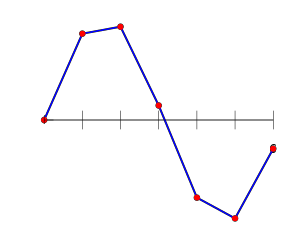
\includegraphics[width=0.5\textwidth]{ArcLength.png}
  \caption*{Approximating the graph $y=f(x)$ by line segments}
\end{figure}
We do this by partitioning the interval $[a,b]$ and approximating the graph $ y = f(x)$ over each partition by a straight line. The length of each small straight line segment equals
\begin{align*}
  \sqrt{\Delta x^2 + \Delta y^2}
\end{align*}
and hence the arc length equals
\begin{align*}
  \lim \limits_{\Delta x \rightarrow 0}  \left(\sum \sqrt{\Delta x^2 + \Delta y^2}\right)
\end{align*}
This looks very close to \eqref{eq:sum_limit}. Next we need to separate a $\Delta x$ term.
\begin{align*}
  \lim \limits_{\Delta x \rightarrow 0} \left(\sum \sqrt{1 + \left(\dfrac{\Delta y}{\Delta x}\right)^2} \Delta x \right)
\end{align*}
This looks exactly like \eqref{eq:sum_limit} with $y$ replaced with $\sqrt{1 + \left(\frac{\Delta y}{\Delta x}\right)^2}$. Finally we notice that
\begin{align*}
  \lim \limits_{\Delta x \rightarrow 0} \dfrac{\Delta y}{\Delta x} = \dfrac{dy}{dx}
\end{align*}
which gives us the formula for the arc length.
\begin{theorem}
  \label{thm:arclength}
  Let $f$ be a differentiable function on the interval $[a,b]$. The arc length of the graph $y = f(x)$ over the interval $[a,b]$ is given by the integral
  \begin{align*}
    \int \limits_a^b \sqrt{1 + \left(\dfrac{dy}{dx} \right)^2}  \: dx
  \end{align*}
\end{theorem}
While the above derivation is not a {\it proof}, it can be converted into a proof using $\sup$'s and $\inf$'s, using the same method we used to prove the Fundamental Theorem of Calculus.

\begin{exercise}
  Using the arc length formula in Theorem \ref{thm:arclength} compute the following:
  \begin{enumerate}
    \item Circumference of a circle of radius r.
    \item Arc length of the parabola $y = x^2$ from 0 to 1.
    \item Arc length of line segment $y = m x$ from $a$ to $b$, where $m$, $a$, $b$ are real numbers. Explain the result geometrically.
  \end{enumerate}
\end{exercise}

\begin{exercise}
  Here we encounter the first example of a {\it naturally occurring} unsolvable integral.
  Find the expression for the arc length of the sine curve $y = \sin x$ from 0 to $a$.
  This integral, called an {\bf elliptic integral}, cannot be algebraically computed.\footnote{Even though elliptic integrals cannot be simplified algebraically, they have deep connections to number theory.
  The impossibility of algebraically evaluating elliptic integrals presents the first obstacle towards a complete understanding of prime numbers!\\
  See: \url{https://en.wikipedia.org/wiki/Elliptic_function}}
\end{exercise}

\begin{exercise}{\bf (Optional)}
  In this problem, you'll need to use the fact that the (curved) surface area of a cylinder is $2 \pi r h$ and the volume is $\pi r^2 h$, where $r$ is the radius and $h$ is the height of the cylinder.
  \begin{figure}[H]
    \centering
    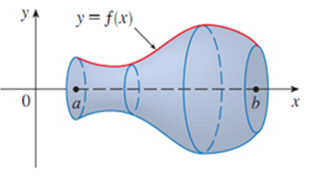
\includegraphics[width=0.5\textwidth]{SurfaceOfRevolution.png}
  \end{figure}
  \end{exercise}
  \begin{enumerate}
    \item Derive the formula for the area of the surface obtained by revolving the curve $y = f(x)$ over the interval $[a,b]$ about the $x$-axis.
   Such a surface is called a {\bf surface of revolution}.
    \item Derive the formula for the volume of the solid obtained by revolving the region under the curve $y = f(x)$ over the interval $[a,b]$ about the $x$-axis.
    Such a solid is called a {\bf solid of revolution}.
  \end{enumerate}
We can do both of these constructions by revolving the curve about the $y$-axis instead of the $x$-axis. In this case, we simply switch $x$ and $y$ and use the function $x=f^{-1}(y)$ instead of $y = f(x)$.\\


\subsection{Differential Equations}
It would be remiss to not mention differential equations while studying applications of calculus.
Calculus was invented by Newton to find solutions to his laws of motion, which are a set of differential equations.

A {\bf differential equation} is any equation involving derivatives $\frac{dy}{dx}$, $\frac{d^2y}{dx^2}$ etc.
Solving a differential equation means finding a function $y = f(x)$ that satisfies the equation.

We've already encountered one very simple differential equation.
The Fundamental Theorem of Calculus is essentially a statement about the solution of a differential equation.
We can rephrase it as saying:\\ {\it The solution to the differential equation
\begin{align*}
  \dfrac{dy}{dx} = g(x)
\end{align*}
is given by
\begin{align*}
  y = \int g(x) \: dx.
\end{align*}
}

In this section, we'll see some examples of differential equations without going into any details.
It is not possible to {\it solve} this differential equation in the same way that we solve algebraic equations. Instead, we {\it guess} a solution and verify it.

\begin{exercise}
  A {\bf separable} differential equation is of the form
  \begin{align*}
    \dfrac{dy}{dx} = f(x) \cdot g(y)
  \end{align*}
  for some functions $f$ and $g$. The solution of this differential equation is given by
  \begin{align*}
    \int \dfrac{1}{g(y)} \: dy  = \int f(x) \: dx
  \end{align*}
  It is called separable because the variables $x$ and $y$ can be ``separated'' i.e. all the terms involving $y$ are on the left hand side and all the terms involving $x$ are on the right hand side. A non-example is $\frac{dy}{dx} = x + y$.

  Find solutions for the following separable differential equations and verify that your solution satisfies the differential equation.
  \begin{multicols}{2}
    \begin{enumerate}
      \item $\dfrac{dy}{dx} = 2y$
      \item $\dfrac{dy}{dx} = xy$
      \item $\dfrac{dy}{dx} = \dfrac{3x^2}{\cos y}$
      \item $\dfrac{dy}{dx} = - \dfrac{y}{x}$
      \item $\dfrac{dy}{dx} = - \dfrac{x}{y}$
      \item $\dfrac{dy}{dx} = e^{-y}(2x - 4) $
    \end{enumerate}
  \end{multicols}
\end{exercise}

\newpage
\begin{exercise}
  The following differential equation is called a {\bf damped harmonic oscillator},
  \begin{align*}
    m \dfrac{d^2y}{dx^2} + c \dfrac{dy}{dx} + k y = 0
  \end{align*}
  where $m$, $k$, and $c$ are constants.
  This differential equation is used to model simple oscillatory systems.
  \begin{enumerate}
    \item Find a number(s) $r$ such that $y=e^{rx}$ solves the differential equation
    \begin{align*}
       \dfrac{d^2y}{dx^2} - 4 y = 0
    \end{align*}
    \item Find a number(s) $r$ such that $y=e^{rx}$ solves the differential equation
    \begin{align*}
       \dfrac{d^2y}{dx^2} + 4 y = 0
    \end{align*}
    \item Find a number(s) $r$ such that $y=e^{rx}$ solves the differential equation
    \begin{align*}
       \dfrac{d^2y}{dx^2} - 2 \dfrac{dy}{dx} + y = 0
    \end{align*}
    For this $r$, verify that $y = x e^{rx}$ is also a solution.
    \item Notice that the three equations have very different kinds of solutions.
    How would you describe the difference between the three equations?
  \end{enumerate}
\end{exercise}

Differential equations in general are very very difficult to solve. Finding solutions to differential equations has been a guiding question for much of modern mathematics. It is still not known whether a solution exists to the differential equation that describes fluid motion.\footnote{See \url{https://en.wikipedia.org/wiki/Navier-Stokes_equations}.} Nevertheless a lot of techniques now exist for solving a variety of differential equations either exactly or numerically.
Differential equations is one of the most active areas of mathematical research today.

  %!TEX root=ClassNotes.tex

\section{Taylor Series}
Taylor series is a technique used to approximate functions using {\it polynomials}.

\begin{definition}
  \label{def:Taylor_series}
For a positive integer $n$, a real number $a$, and an infinitely differentiable function $f$, the {\bf n$^{th}$ Taylor polynomial/approximation centered at $a$}, denoted $T_nf (x)$, is a degree $n$ polynomial defined as\\
  \begin{align*}
    T_nf (x) &= f(a)
    + f'(a) \cdot \dfrac{(x-a)}{1}
    + f''(a) \cdot \dfrac{(x-a)^2}{2!}
    + \dots
    + f^{(n)}(a) \cdot \dfrac{(x-a)^n}{n!}\\
  \end{align*}
  where $f^{(n)}(a)$ denotes the $n^{th}$ derivative of $f$ at $a$.\footnote{Recall that $n! = n \cdot (n-1) \cdot (n-2) \cdots 2 \cdot 1 $.}
The limit $n \rightarrow \infty$ of the above series is called the {\bf Taylor series $Tf(x)$}.\\
\begin{align*}
  Tf(x) &= f(a)
  + f'(a) \cdot \dfrac{(x-a)}{1}
  + f''(a) \cdot \dfrac{(x-a)^2}{2!}
  + f^{(3)}(a) \cdot \dfrac{(x-a)^3}{3!}
  + \dots\\
\end{align*}
\end{definition}

\begin{remark}
  The Taylor series defined above is just a {\it formal series}.
  It is not always possible to plug in a value for $x$ because of convergence issues.
  We'll discuss this in the later sections.
\end{remark}

We'll mostly be interested in the Taylor series centered at $a = 0$, \\
\begin{align*}
  Tf(x)
  &=
  f(0)
  + f'(0) \cdot \dfrac{x}{1}
  + f''(0) \cdot \dfrac{x^2}{2!}
  + f^{(3)}(0) \cdot \dfrac{x^3}{3!}
  + \dots\\
\end{align*}
In this case, $Tf(x)$ is called the $n^{th}$ {\bf Maclaurin series}.



\begin{exercise}
  For each of the following functions compute $f^{(n)}(0)$, for positive integers $n$, and use these to compute the Maclaurin series.
  \begin{multicols}{2}
  \begin{enumerate}
    \item $e^x$
    \item $\sin x$
    \item $\cos x$
    \item $\ln {(1+x)}$
    \item $\dfrac{1}{1-x}$
    \item (Optional) $\tan^{-1} x$
  \end{enumerate}
  \end{multicols}
\end{exercise}

\begin{exercise}
  This problem explains why the Definition \ref{def:Taylor_series} is the ``correct'' definition for Taylor series.
  \begin{enumerate}
    \item Let $f(x) = x^k$. Compute $T_n f(x)$ centered at $0$ for
    \begin{enumerate}
      \item $n < k$
      \item $n \ge k$
    \end{enumerate}
    \item More generally, let
    \begin{align*}
      f(x) = a_0 + a_1 x + a_2 x^2 + \dots + a_k x^k
    \end{align*}
    Using the previous part, compute $T_n f(x)$ for
    \begin{enumerate}
      \item $n < k$
      \item $n \ge k$
    \end{enumerate}
     What is the Maclaurin series for this $f(x)$?
  \end{enumerate}
\end{exercise}
The above statement is more generally for all Taylor series centered at any point $a$.
\begin{exercise}{\bf (Optional)}
  Show that the Taylor series of $f(x) = x^n$, centered at a real number $a$, equals $x^n$. Argue that this is more generally true for an arbitrary polynomial $f(x)$.
\end{exercise}

\subsection{Remainder Term}
As mentioned earlier, Definition \ref{def:Taylor_series} defines a \textit{formal series} and it not possible to make sense of $Tf(x)$ for a real number $x$.
The two important questions that we need to answer are:
\begin{enumerate}
  \item  Does the limit $\lim \limits_{n \rightarrow \infty}T_n f(x)$ exist?
  \item Does the limit $\lim \limits_{n \rightarrow \infty}T_n f(x)$ equal $f(x)$?
\end{enumerate}
Unless the answer to both the questions is {\it yes} it is not possible to use Taylor polynomials for approximating the function $f(x)$.

Both the questions are in generally difficult to answer.
To tackle the first question we need techniques from series and sequences.
In this section, we'll focus on answering the second question which can be done using basic Calculus.


\begin{definition}
  For a smooth function $f$ and real numbers $x$, $a$, the {\bf $n^{th}$ error term} or the {\bf $n^{th}$ remainder term $R_nf(x)$} is defined as
  \begin{align*}
    R_nf(x)
    &= f(x) - T_nf(x)
  \end{align*}
  where $T_n f(x)$ is the $n^{th}$ Taylor approximation of $f$ centered at $a$, so that $f(x) = T_nf(x) + R_nf(x)$.
Thus we can say that
\begin{align*}
  \lim \limits_{n \rightarrow \infty}T_n f(x) = f(x)
\end{align*}
if and only if
\begin{align*}
  \lim \limits_{n \rightarrow \infty}R_n f(x) = 0.
\end{align*}
\end{definition}

\newpage

The following Theorem allows us to compute this remainder term using integrals.
\begin{theorem}
  \label{thm:remainder_term}
  With the notation as above, the remainder term is given by
  \begin{align*}
    R_nf(x) = \dfrac{1}{n!} \cdot \int_a^x {(x-t)^n \cdot {f^{(n+1)}(t)} } \: dt
  \end{align*}
\end{theorem}

\begin{exercise}
  \begin{enumerate}
    \item Using integration by parts (if necessary), compute
    \begin{enumerate}
      \item $\int_0^x {f'(t)} \: dt$
      \item $\int_0^x (x-t) \cdot {f''(t)} \: dt$
      \item $\int_0^x (x-t)^2 \cdot {f^{(3)}(t)} \: dt$
    \end{enumerate}
    \item{\bf (Optional)} By repeatedly applying integration by parts, prove that
    \begin{align*}
      \dfrac{1}{n!} \cdot \int_0^x {(x-t)^n \cdot {f^{(n+1)}(t)}} \: dt
    \end{align*}
    equals
    \begin{align*}
      f(x) - \left( f(0)
      + f'(0) \cdot \dfrac{x}{1}
      + f''(0) \cdot \dfrac{x^2}{2!}
      + \dots
      + f^{(n)}(0) \cdot \dfrac{x^n}{n!}
      \right)
    \end{align*}
    thereby proving Theorem \ref{thm:remainder_term} for $a=0$.
  \end{enumerate}
\end{exercise}

\begin{exercise}{\bf (Optional)}
  Prove Theorem \ref{thm:remainder_term} for arbitrary real number $a$.
\end{exercise}


\newpage
\subsection{Computing using Taylor Series}
We can use the Taylor series (centered at 0) to do computations if
\begin{enumerate}
  \item we can compute all the derivatives $f^{(n)}(0)$ for all positive integers $n$
  \item $ \lim \limits_{n \rightarrow \infty}R_n f(x) = 0$.
\end{enumerate}
The condition $ \lim \limits_{n \rightarrow \infty}R_n f(x) = 0$ is highly non-trivial and not checking it leads to absurd results.

\begin{exercise}
  Let $f(x) = \dfrac{1}{1-x}$.
  What happens to the value of the Maclaurin series $Tf(x)$ for $x=2$? What is $f(2)$?
\end{exercise}
For $f(x) = \dfrac{1}{1-x}$ we can show that $ \lim \limits_{n \rightarrow \infty}R_n f(2) = \infty$ (and not 0) and hence the difference between the Taylor series $Tf(2)$ and the function $f(2)$ blows up to infinity.
In the next section, we'll prove the following theorem which says that this does not happen for exponential and trigonometric functions.
\begin{theorem}
  \label{thm:Taylor_series_exponential}
  If $f(x) = e^x$, $\sin x$, and $\cos x$, then $\lim \limits_{n \rightarrow \infty}R_n f(x) = 0$ for \textit{all real numbers} x.
\end{theorem}

Hence, for all real numbers $x$, $\lim \limits_{n \rightarrow \infty}T_n f(x) = f(x)$ for exponential and trigonometric functions and we can use the Taylor series to approximate.

\begin{exercise}
  Use the Maclaurin series of $e^x$ to compute the value of $e$ correct up to 2 decimal places.
\end{exercise}

\begin{exercise}
  \begin{enumerate}
    \item Theorem \ref{thm:Taylor_series_exponential} is also true for $\tan^{-1} x$, the proof is easy but technical. The Maclaurin series of $\tan^{-1} x$ is given by
    \begin{align*}
      x - \dfrac{x^3}{3} + \dfrac{x^5}{5} - \dfrac{x^7}{7} + \dfrac{x^9}{9} + - \dots
    \end{align*}
    Using this find an expression (as an infinite sum) for $\pi$.\hint{Use $x = 1$.}
    \item Use the first 10 terms of this sum to find an approximate value for $\pi$.
    This method for computing $\pi$ is not used in practice as the \textit{rate of convergence} of the Maclaurin series is very slow.
  \end{enumerate}
\end{exercise}

\begin{exercise}
  Theorem \ref{thm:Taylor_series_exponential} is true even if $x$ is a complex number (the proof requires complex analysis).
  Compute the Taylor series of $e^{i\theta}$, $\cos \theta$, $\sin \theta$. Use these to prove the {\it Euler's identity},
\begin{align*}
    e^{i\theta} &= \cos \theta + i \sin \theta
\end{align*}
\end{exercise}



\subsection{Estimating the Remainder Term}
Finally, we  want to prove Theorem \ref{thm:Taylor_series_exponential}.

\begin{exercise} {\bf (Optional)}
  Let $x$ be a positive real number.
   For each of the following functions $f(x)$, show that there is a constant $M$ such that for all $ t \in (0,x)$  and all positive integers $n$ we have $|f^{(n)}(t)| < M$. (Note that $M$ can depend on $x$ but not on $n$ or $t$.)
   \begin{multicols}{2}
     \begin{enumerate}
       \item $e^x$
       \item $\sin x$
       \item $\cos x$
     \end{enumerate}
   \end{multicols}
\end{exercise}
Using the above problem, the proof of Theorem \ref{thm:Taylor_series_exponential} will be complete once we prove the following Proposition.
\begin{prop}
  Let $x$ be a positive real number. If there is a real number $M$ such that for all $ t \in (0,x)$  and all positive integers $n$ we have $|f^{(n)}(x)| < M$ then $R_n f(x) \rightarrow 0$ as $n \rightarrow \infty$.
\end{prop}
\begin{proof}
  By definition,
  \begin{align*}
    R_n f(x) = \dfrac{1}{n!} \cdot \int_0^x {(x-t)^n \cdot {f^{(n+1)}(t)}} \: dt
  \end{align*}
  Because $(x-t)^n < x^n$ and $|f^{(n+1)}(t)| < M$ for all $0 < t < x$  and all positive integers $n$, we get
  \begin{align*}
    |R_n f(x)|
    &=
    \left|\dfrac{1}{n!} \cdot \int_0^x {(x-t)^n \cdot {f^{(n+1)}(t)}} \: dt \right|\\
    &< \left|\dfrac{1}{n!} \cdot \int_0^x x^n \cdot M \: dt \right| \\
    &=  \left|\dfrac{1}{n!} \cdot x^n \cdot M \int_0^x 1 \: dt \right| \\
    &=  \left|\dfrac{1}{n!} \cdot x^n \cdot M x \right| \\
    &= \dfrac{M x^{n+1}}{n!}
  \end{align*}
  One can show that for any real number $x$, $\lim \limits_{n \rightarrow \infty} x^{n+1} / n! = 0$ (this is easy, see if you can work out the details) so that
\begin{align*}
    \lim \limits_{n \rightarrow \infty} |R_n f(x)|
    &<
    \lim \limits_{n \rightarrow \infty} \dfrac{M x^{n+1}}{n!}
    \\
    &= {M}\cdot \lim \limits_{n \rightarrow \infty} \dfrac{x^{n+1}}{n!} \\
    &= M \cdot 0 = 0
\end{align*}
\end{proof}

To summarize, Taylor series provides us a tool for approximating functions using polynomials (in the cases where the remainder term tends to 0).
This is a very common technique in analysis: we try to approximate a function by a series of simpler functions and show that the difference between the two tends to 0.
Fourier series, for example, does this using trigonometric functions.


  %!TEX root=ClassNotes.tex

\appendix
\section{Table of Integrals}
\setlength\extrarowheight{5pt}
\begin{center}
  \begin{tabular}{|l|l|l|l|}
    \hline
    ${\bf f(x)}$ & ${\bf f'(x)}$ & ${\bf g(x)}$ & ${\bf \int g(x) \: dx + c}$ \\ \hline
    $x^n$ & $n x^{n - 1}$ & $x^{n-1} \mbox{ if } n \neq 0$ & ${x^n}/{n}$ \\ \hline
    $\ln x$ & $1/x$ & $1/x$ & $\ln x$ \\
    $e^x$ & $e^x$ & $e^x$ & $e^x$ \\ \hline
    $\sin^{-1} x$ & $1/\sqrt{1-x^2}$ & $1/\sqrt{1-x^2}$ & $\sin^{-1} x$ \\
    $\tan^{-1} x$ & $1/{(1+x^2)}$ & $1/{(1+x^2)}$ & $\tan^{-1} x$ \\ \hline
    $\sin x$ & $\cos x$ & $\cos x$ & $\sin x$ \\
    $\cos x$ & $-\sin x$ & $\sin x$ & $-\cos x$ \\
    $\tan x$ & $\sec^2 x$ & $\sec^2 x$ & $\tan x$ \\
		$\sec x$ & $\sec x \tan x$ & $ \sec x \tan x$ & $\sec x$ \\\hline
		& & $\tan x$ & $- \ln (\cos x)$\\
		& & $\cot x$ & $ \ln (\sin x)$\\
		& & $\sec x$ & $ \ln (\sec x + \tan x)$\\
		& & $\csc x$ & $ -\ln (\csc x + \cot x)$ \\\hline
    & & $\sec^3 x$ &  $\frac{1}{2} \cdot \left(\tan x \sec x + \ln (\sec x + \tan x)\right)$\\\hline
	\end{tabular}
\end{center}

\vspace{2em}
	\section{Trig identities}
	\begin{align*}
			\sin^2 \theta + \cos^2 \theta &= 1 \\
			\sec^2 \theta &= 1 + \tan^2 \theta
	\end{align*}
	\begin{align*}
		\sin (2 \theta)
			&= 2 \sin \theta \cos \theta
	\end{align*}
\begin{align*}
		\cos(2 \theta)
		&= \cos^2 \theta - \sin^2 \theta \\
		&= 2 \cos^2 \theta - 1 \\
		&= 1 - 2 \sin^2 \theta
\end{align*}


\end{document}
